\documentclass[11pt,twocolumn]{article}

% ==================================================================
%  Assessing the Reliability of ML Atmospheric Retrievals
%  Compile:  tectonic PAPER.tex   (or pdflatex twice)
%  Figures are read from the figures/ subfolder next to this file.
% ==================================================================
\usepackage[margin=0.8in]{geometry}
\usepackage{booktabs}
\usepackage{amsmath}
\usepackage{amssymb}
\usepackage{array}
\usepackage{graphicx}
\graphicspath{{figures/}{./}}
\usepackage{siunitx}
\usepackage{microtype}
\usepackage[hidelinks]{hyperref}
\usepackage{caption}
\captionsetup{font=small,labelfont=bf,skip=5pt}

% Numeric \cite for natbib-style commands (no natbib dependency).
\newcommand{\citep}[1]{\cite{#1}}
\newcommand{\citet}[1]{\cite{#1}}

\newcommand{\um}{\,$\mu$m}
\newcommand{\co}{$\mathrm{CO_2}$}
\newcommand{\ot}{$\mathrm{O_2}$}
\newcommand{\oth}{$\mathrm{O_3}$}
\newcommand{\ch}{$\mathrm{CH_4}$}
\newcommand{\wat}{$\mathrm{H_2O}$}
\newcommand{\ntwo}{$\mathrm{N_2}$}

% Float placement: reduce congestion / overlap of stacked floats.
\renewcommand{\topfraction}{0.9}
\renewcommand{\bottomfraction}{0.8}
\renewcommand{\textfraction}{0.07}
\renewcommand{\floatpagefraction}{0.75}
\renewcommand{\dbltopfraction}{0.9}
\renewcommand{\dblfloatpagefraction}{0.8}
\setcounter{topnumber}{3}
\setcounter{bottomnumber}{2}
\setcounter{totalnumber}{5}
\setlength{\textfloatsep}{14pt plus 3pt minus 3pt}
\setlength{\dbltextfloatsep}{16pt plus 3pt minus 3pt}
\setlength{\intextsep}{12pt plus 3pt minus 3pt}

% Placeholder box for architecture diagrams to be drawn later.
\newcommand{\diagramplaceholder}[1]{%
  \setlength{\fboxsep}{0pt}%
  \framebox[\linewidth]{\parbox[c][#1][c]{0.94\linewidth}{%
    \centering\itshape\small Architecture schematic to be inserted}}%
}

\title{\textbf{Assessing the Reliability of Machine-Learning Atmospheric
Retrievals with Real Solar-System Spectra}}
\author{}
\date{July 2026}

\begin{document}

\makeatletter
\twocolumn[
  \begin{@twocolumnfalse}
    \maketitle
    \begin{abstract}
    \noindent
    Machine-learning retrieval is often proposed as a fast substitute for
    Bayesian atmospheric inference, but almost every published model is trained
    and tested only on synthetic spectra, so its behaviour on real observations
    is unknown. We evaluate six neural architectures (\num{520000} to
    \num{36000000} parameters) trained on a synthetic library of terrestrial
    reflected-light spectra and tested, without retraining, on real telescope
    spectra of 19 Solar-System bodies. Every accuracy figure is reported at two
    operating points: a noiseless ceiling and a realistic single exposure
    ($\alpha{=}1$, an 8\,h integration). The best model reaches a covered-gas
    $R^2$ of $0.78$ at the ceiling but $0.13$ at $\alpha{=}1$, a factor-of-six
    gap. On the real spectra the models detect methane as well as a
    one-parameter physics ruler, but assign more oxygen to the airless Moon than
    to Earth, a fabrication we trace to the training-set label prior rather than
    to any architecture. Model size does not improve accuracy, transfer to a
    different simulator degrades, and calibrated uncertainty holds only
    in-distribution. We frame the study around these limitations: synthetic
    accuracy is a weak predictor of real-world reliability, and physical controls
    such as airless-body false-positive tests and continuum nulling are needed to
    tell the two apart.
    \end{abstract}
    \vspace{1.4em}
  \end{@twocolumnfalse}
]
\makeatother

% ==================================================================
\section{Introduction}
% ==================================================================

Characterising the atmospheres of rocky planets is central to the search for
life beyond the Solar System. The gases present in an atmosphere, their
abundances, and the chemical disequilibria between them are the primary remote
evidence for whether a planet's surface chemistry could be biological. Oxygen
and its photochemical product ozone, together with methane, are the canonical
targets: their simultaneous presence is hard to sustain without a continual
biological source. That same importance makes them the most costly to get wrong.
An abiotic process, or an analysis artefact, that mimics oxygen would register as
a false detection of life, so the reliability of a retrieval matters as much as
its nominal accuracy.

Future direct-imaging missions are expected to rely on reflected-light
spectroscopy, one of the few routes to Earth-like planets around Sun-like stars
that transit spectroscopy cannot easily reach \citep{gilbert2024,damiano2020}.
Interpreting such spectra, a task known as atmospheric \emph{retrieval}, is
traditionally posed as Bayesian inference: a forward model is evaluated
repeatedly against the observation until the posterior over atmospheric
parameters is characterised. The approach is statistically principled but
expensive. Nested-sampling retrievals typically need between \num{20000} and
\num{60000} forward-model evaluations, and Bayesian schemes more generally
require $10^{5}$ to $10^{6}$ evaluations, corresponding to hours of wall-clock
time per spectrum \citep{ardevol2022,nixon2020}. As direct-imaging surveys begin
to return larger samples of candidate planets, this cost becomes a bottleneck.

Supervised machine learning offers a faster route. A model learns the mapping
from spectrum to composition from a synthetic training library and then analyses
a new observation in a single forward pass, reducing per-spectrum inference from
CPU-hours to milliseconds \citep{waldmann2016,marquez2018,soboczenski2018}. A
common limitation runs through this literature: with few exceptions the models
are trained \emph{and} evaluated on synthetic spectra produced by a single
forward model, so strong performance on held-out synthetic data measures
self-consistency with the simulator rather than fidelity to nature. This paper
takes that limitation as its subject. Using frozen, already-trained models, and
without any retraining, we ask four questions. How large does a retrieval model
need to be before accuracy saturates? How does the reported accuracy depend on
exposure time and spectral resolution? How does a model behave on spectra from a
different simulator? And, most importantly, how does it behave on real telescope
spectra whose ground truth is known independently of any simulator?

To answer the last question we assemble a real-data validation set of 19
Solar-System bodies observed in reflected light, including 11 airless bodies that
serve as a false-positive control. The main finding is a gap: a model can post a
strong synthetic benchmark and still fail on real spectra, most starkly by
reporting abundant oxygen on bare rock. The remaining results characterise where
and why learned retrieval breaks down, and what inexpensive controls expose the
failure. Throughout, we report every accuracy figure at two operating points, a
noiseless ceiling and a realistic single exposure, so that the optimism of the
synthetic-only number is visible directly rather than hidden.

% ==================================================================
\section{Related work}
% ==================================================================

Learned atmospheric retrieval has progressed steadily from simple to expressive
models. Waldmann \citep{waldmann2016} introduced deep networks for recognising
spectral patterns; M\'arquez-Neila et al.\ \citep{marquez2018} used a random
forest to retrieve a hot-Jupiter atmosphere and compared its posterior against a
Bayesian one; Soboczenski et al.\ \citep{soboczenski2018} and Cobb et al.\
\citep{cobb2019} added Bayesian deep networks and ensembles to attach
uncertainty to terrestrial retrievals. Generative and simulation-based methods
followed, including generative adversarial networks \citep{zingales2018} and
neural posterior estimation with normalizing flows, the latter winning the 2023
Ariel Data Challenge \citep{vasist2023,aubin2023}. Nixon \& Madhusudhan
\citep{nixon2020} showed that, given enough training data, supervised models can
match nested-sampling parameter estimates at a fraction of the cost, and
Ard\'evol Mart\'inez et al.\ \citep{ardevol2022} compared convolutional networks
against nested sampling on transmission spectra.

Two threads matter for the present work. First, uncertainty tends to be
under-dispersed: learned posteriors are often narrower than the Bayesian
reference \citep{marquez2018}, which motivates the calibrated intervals we adopt.
Second, real-data validation is rare. Most studies remain within a single
simulator, so the domain shift to real observations, which includes instrumental
systematics, geometry, and cloud, is left untested. Table~\ref{tab:related}
places our study among representative prior work; it differs chiefly in being
validated on real telescope spectra with independent ground truth.

\begin{table*}[t]
\centering
\caption{Representative machine-learning studies for exoplanet atmospheric
retrieval. The present work extends synthetic-only evaluation with a real-data
validation set of Solar-System bodies.}
\label{tab:related}
\small
\begin{tabular}{@{}p{3.8cm}p{4.6cm}p{4.4cm}c@{}}
\toprule
Study & Model family & Data regime & Real data? \\
\midrule
Waldmann (2016) & Deep belief network & Synthetic transmission & No \\
M\'arquez-Neila et al.\ (2018) & Random forest & Single hot Jupiter & Partial \\
Soboczenski et al.\ (2018) & Bayesian DNN (MC dropout) & Synthetic terrestrial (PSG) & No \\
Cobb et al.\ (2019) & Ensemble of Bayesian NNs & Synthetic terrestrial & No \\
Nixon \& Madhusudhan (2020) & Multiple supervised models & Synthetic, cross-compared & No \\
Ard\'evol Mart\'inez et al.\ (2022) & CNN vs.\ nested sampling & Synthetic transmission & Partial \\
Vasist et al.\ (2023) & Normalizing-flow NPE & Synthetic (Ariel) & No \\
This work & Six architectures (0.52--36M) & Synthetic PSG + Solar System & Yes (19 bodies) \\
\bottomrule
\end{tabular}
\end{table*}

% ==================================================================
\section{Data}
% ==================================================================

\subsection{Synthetic training library}

Training uses the INARA library \citep{zorzan2025}, a set of reflected-light
spectra of rocky planets generated with the NASA Planetary Spectrum Generator
(PSG) \citep{villanueva2018}, the forward model behind the reference terrestrial
data sets in this field. We use \num{99305} spectra, split \num{88271} for
training and \num{11034} for a held-out test set. Each spectrum spans
$0.2$--$2.0$\um{} at native resolving power $R\!\approx\!1900$ (\num{4378}
wavelength bins) and carries a 12-species volume-mixing-ratio (VMR) label on the
simplex (\wat, \co, \ot, \ntwo, \ch, $\mathrm{N_2O}$, CO, \oth,
$\mathrm{SO_2}$, $\mathrm{NH_3}$, $\mathrm{C_2H_6}$, $\mathrm{NO_2}$). Five of
these, \wat, \co, \ot, \ch, and \oth, produce measurable absorption in the
reflected-light band, and we refer to them as the \emph{covered gases}; headline
$R^2$ values average over these five unless stated otherwise. To probe whether a
model has memorised the idiosyncrasies of one simulator, we also generate
held-out sets of \num{2000} spectra each with two independent forward models,
TauREx and petitRADTRANS (pRT), on the same wavelength grid
(Section~\ref{sec:crosssim}).

\subsection{Real validation set}
\label{sec:realdata_data}

The validation data are the focus of this work. We use the Solar-System
reflectance catalogue of Madden \& Kaltenegger \citep{madden2018}, which provides
disc-integrated geometric-albedo spectra $A_g(\lambda)$ for 19 bodies whose
atmospheric compositions are known independently, from decades of in-situ and
remote study rather than from any simulator. This makes them a clean external
test of models trained only on synthetic data: the answer key was never seen in
training and does not share the simulator's biases. We group the bodies to probe
distinct failure modes.

\emph{Terrestrial bodies with atmospheres} (Earth, Venus, Mars, Titan) test
whether known gases are recovered. \emph{Giant planets} (Jupiter, Saturn,
Uranus, Neptune) test behaviour on atmospheres far outside the rocky training
distribution. \emph{Airless bodies} (the Moon, Mercury, and nine icy or rocky
moons and dwarf planets) are a false-positive control: a body with no atmosphere
that is nonetheless assigned a gas abundance exposes fabrication directly, since
the model must then be reciting its training prior rather than reading absorption
features. The catalogue also contains a matched Earth/Moon pair observed on the
same night with the same instrument at the same resolving power, which isolates
composition from every observational confound and is the single cleanest test in
the set.

The bodies span a wide range of native resolving power, from $R\!\approx\!12$ to
$R\!\approx\!867$. Because reflected-light features blend below a threshold, we
record each body's effective $R$ and treat quantitative abundance retrieval as
valid only where $R\!\ge\!400$; below that we restrict the analysis to detection
statistics. This is not a modelling choice but a physical limit, and it makes
some bodies (Venus and Mars at $R\!\approx\!22$) unusable for quantitative
retrieval regardless of the method.

% ==================================================================
\section{Methodology}
% ==================================================================

\subsection{Input representation and noise}
\label{sec:input}

The models operate on the planet-to-star contrast rather than on absolute flux,
which removes the dependence on stellar luminosity and system distance and lets
the network learn atmospheric properties rather than observational scaling. The
stellar flux is recovered from the combined star-planet spectrum and the isolated
planetary spectrum, and the noiseless contrast is
$C(\lambda)=F_p(\lambda)/F_\star(\lambda)$.

The INARA library ships a per-wavelength $1\sigma$ noise column, a realistic
LUVOIR-class photon-noise estimate. Most prior work discards it and trains on
noiseless spectra, which is one reason synthetic accuracy overstates real
performance: a model tuned on noiseless data is never asked to cope with the
photon budget it will face in practice. We instead build our noise model on this
column. Rather than fixing a single noisy data set, we inject noise dynamically
during training. With a nominal exposure $t_\mathrm{nom}=8$\,h (a LUVOIR-class
integration), we define an exposure factor and draw a fresh noisy realisation
each epoch,
\begin{equation}
\alpha=\sqrt{t_\mathrm{exp}/t_\mathrm{nom}},\qquad
\tilde{C}(\lambda)=C(\lambda)+\frac{\sigma_C(\lambda)}{\alpha}\,\mathcal{N}(0,1),
\end{equation}
where $\sigma_C(\lambda)=\sigma_\mathrm{noise}(\lambda)/F_\star(\lambda)$, so
that the noise falls as $1/\alpha$ with integration time in accordance with
photon-counting statistics. Here $\alpha{=}1$ is a single realistic 8\,h
exposure; $\alpha{\gg}1$ mimics stacking many exposures and approaches the
noiseless limit. Because a model trained across a range of $\alpha$ sees the same
atmosphere at many noise levels, sweeping $\alpha$ at test time traces the entire
photon-limited accuracy curve. The practical consequence is that every accuracy
number must be quoted with its $\alpha$: the same network can look strong or weak
depending only on the assumed exposure, and reporting the noiseless value alone
is the central source of optimism this paper warns against.

Each spectrum is presented as two channels: the noisy contrast
$\tilde{C}(\lambda)$, and the stellar signal-to-noise ratio
$\mathrm{SNR}_\star(\lambda)=\alpha\,F_\star(\lambda)/\sigma_\mathrm{noise}
(\lambda)$, which tells the network how trustworthy each wavelength is. Both
channels are compressed with the inverse hyperbolic sine,
$x_\mathrm{norm}=\operatorname{asinh}(x)=\ln(x+\sqrt{x^2+1})$, which tames the
roughly 13-decade dynamic range while preserving low-intensity structure. The
full \num{4378}-bin spectrum is passed to the neural networks; a 64-bin pooled
representation is used only for the classical baselines
(Section~\ref{sec:baselines}).

For real spectra the catalogue provides geometric albedo, whereas the models
expect the two-channel contrast input. For each body we convert $A_g(\lambda)$ to
a planetary contrast under an explicit Earth-analogue geometry (1\,AU orbit,
Solar-type host, full phase) and place it on the training wavelength grid. The
SNR channel is set to the nominal $\alpha{=}1$ stellar profile, identical for all
bodies, so no per-body information leaks through it. This conversion is an
assumption, not a measurement, and we treat it as part of the test: any retrieval
that depends sensitively on it is flagged, and detection statistics are computed
at matched resolution so that resolving power cannot act as a confound.

\subsection{Training and evaluation setup}
\label{sec:setup}

All tracks are trained under one harness and a shared budget: the same optimiser,
batch size, learning rate, and a 48-epoch schedule, with fresh photon noise drawn
each epoch as above. Except for the deliberately large convolutional baseline,
every model is kept below 2M parameters so that the family can be trained and
audited on modest hardware and compared on an equal footing. Results in this
paper come from single-seed runs; we note where that limits the strength of a
conclusion, and a multi-seed study is left to future work. Unless stated, all
numbers are computed from frozen checkpoints with no retraining, including every
real-data and inference-time-correction result.

\subsection{Architectures}
\label{sec:arch}

We evaluate five distinct architectures; a sixth track is byte-identical to the
convolutional baseline and is reported only for continuity. The models are
summarised briefly here, and the counterfactual model is described separately in
Section~\ref{sec:causal}.

\paragraph{Large CNN baseline (\texttt{original1dcnn}, 36M).} A deliberately
large model. Prior terrestrial-retrieval networks used millions of parameters
(Soboczenski et al.\ $\sim$18M; other studies exceed 5M), so we reproduce a
36M-parameter deep 1-D CNN with a large fully connected head. Its role is to test
directly whether brute-force capacity is what drives accuracy, and it anchors the
upper end of the size range.

\paragraph{Compact CNN (\texttt{optimized1dcnn}, 1.2M).} A 1-D CNN with batch
normalisation, progressive kernel sizes, and adaptive pooling, giving a receptive
field comparable to the large baseline at a fraction of the size.

\paragraph{Transformer backbone (\texttt{transformerarch}, 0.52M).} A
convolutional down-sampling stem ($\times 8$) feeds a two-layer Transformer
encoder, global average pooling, and an MLP head (Figure~\ref{fig:transdiag}).
The \texttt{causal} track shares this exact backbone and differs only in training
objective, so comparing the two isolates the effect of the augmentation.

\paragraph{Wide causal net (\texttt{causal\_xl}, 2M).} A wider, deeper
counterfactual backbone, included to test whether extra capacity on the causal
track helps.

\begin{figure}[t]
\centering
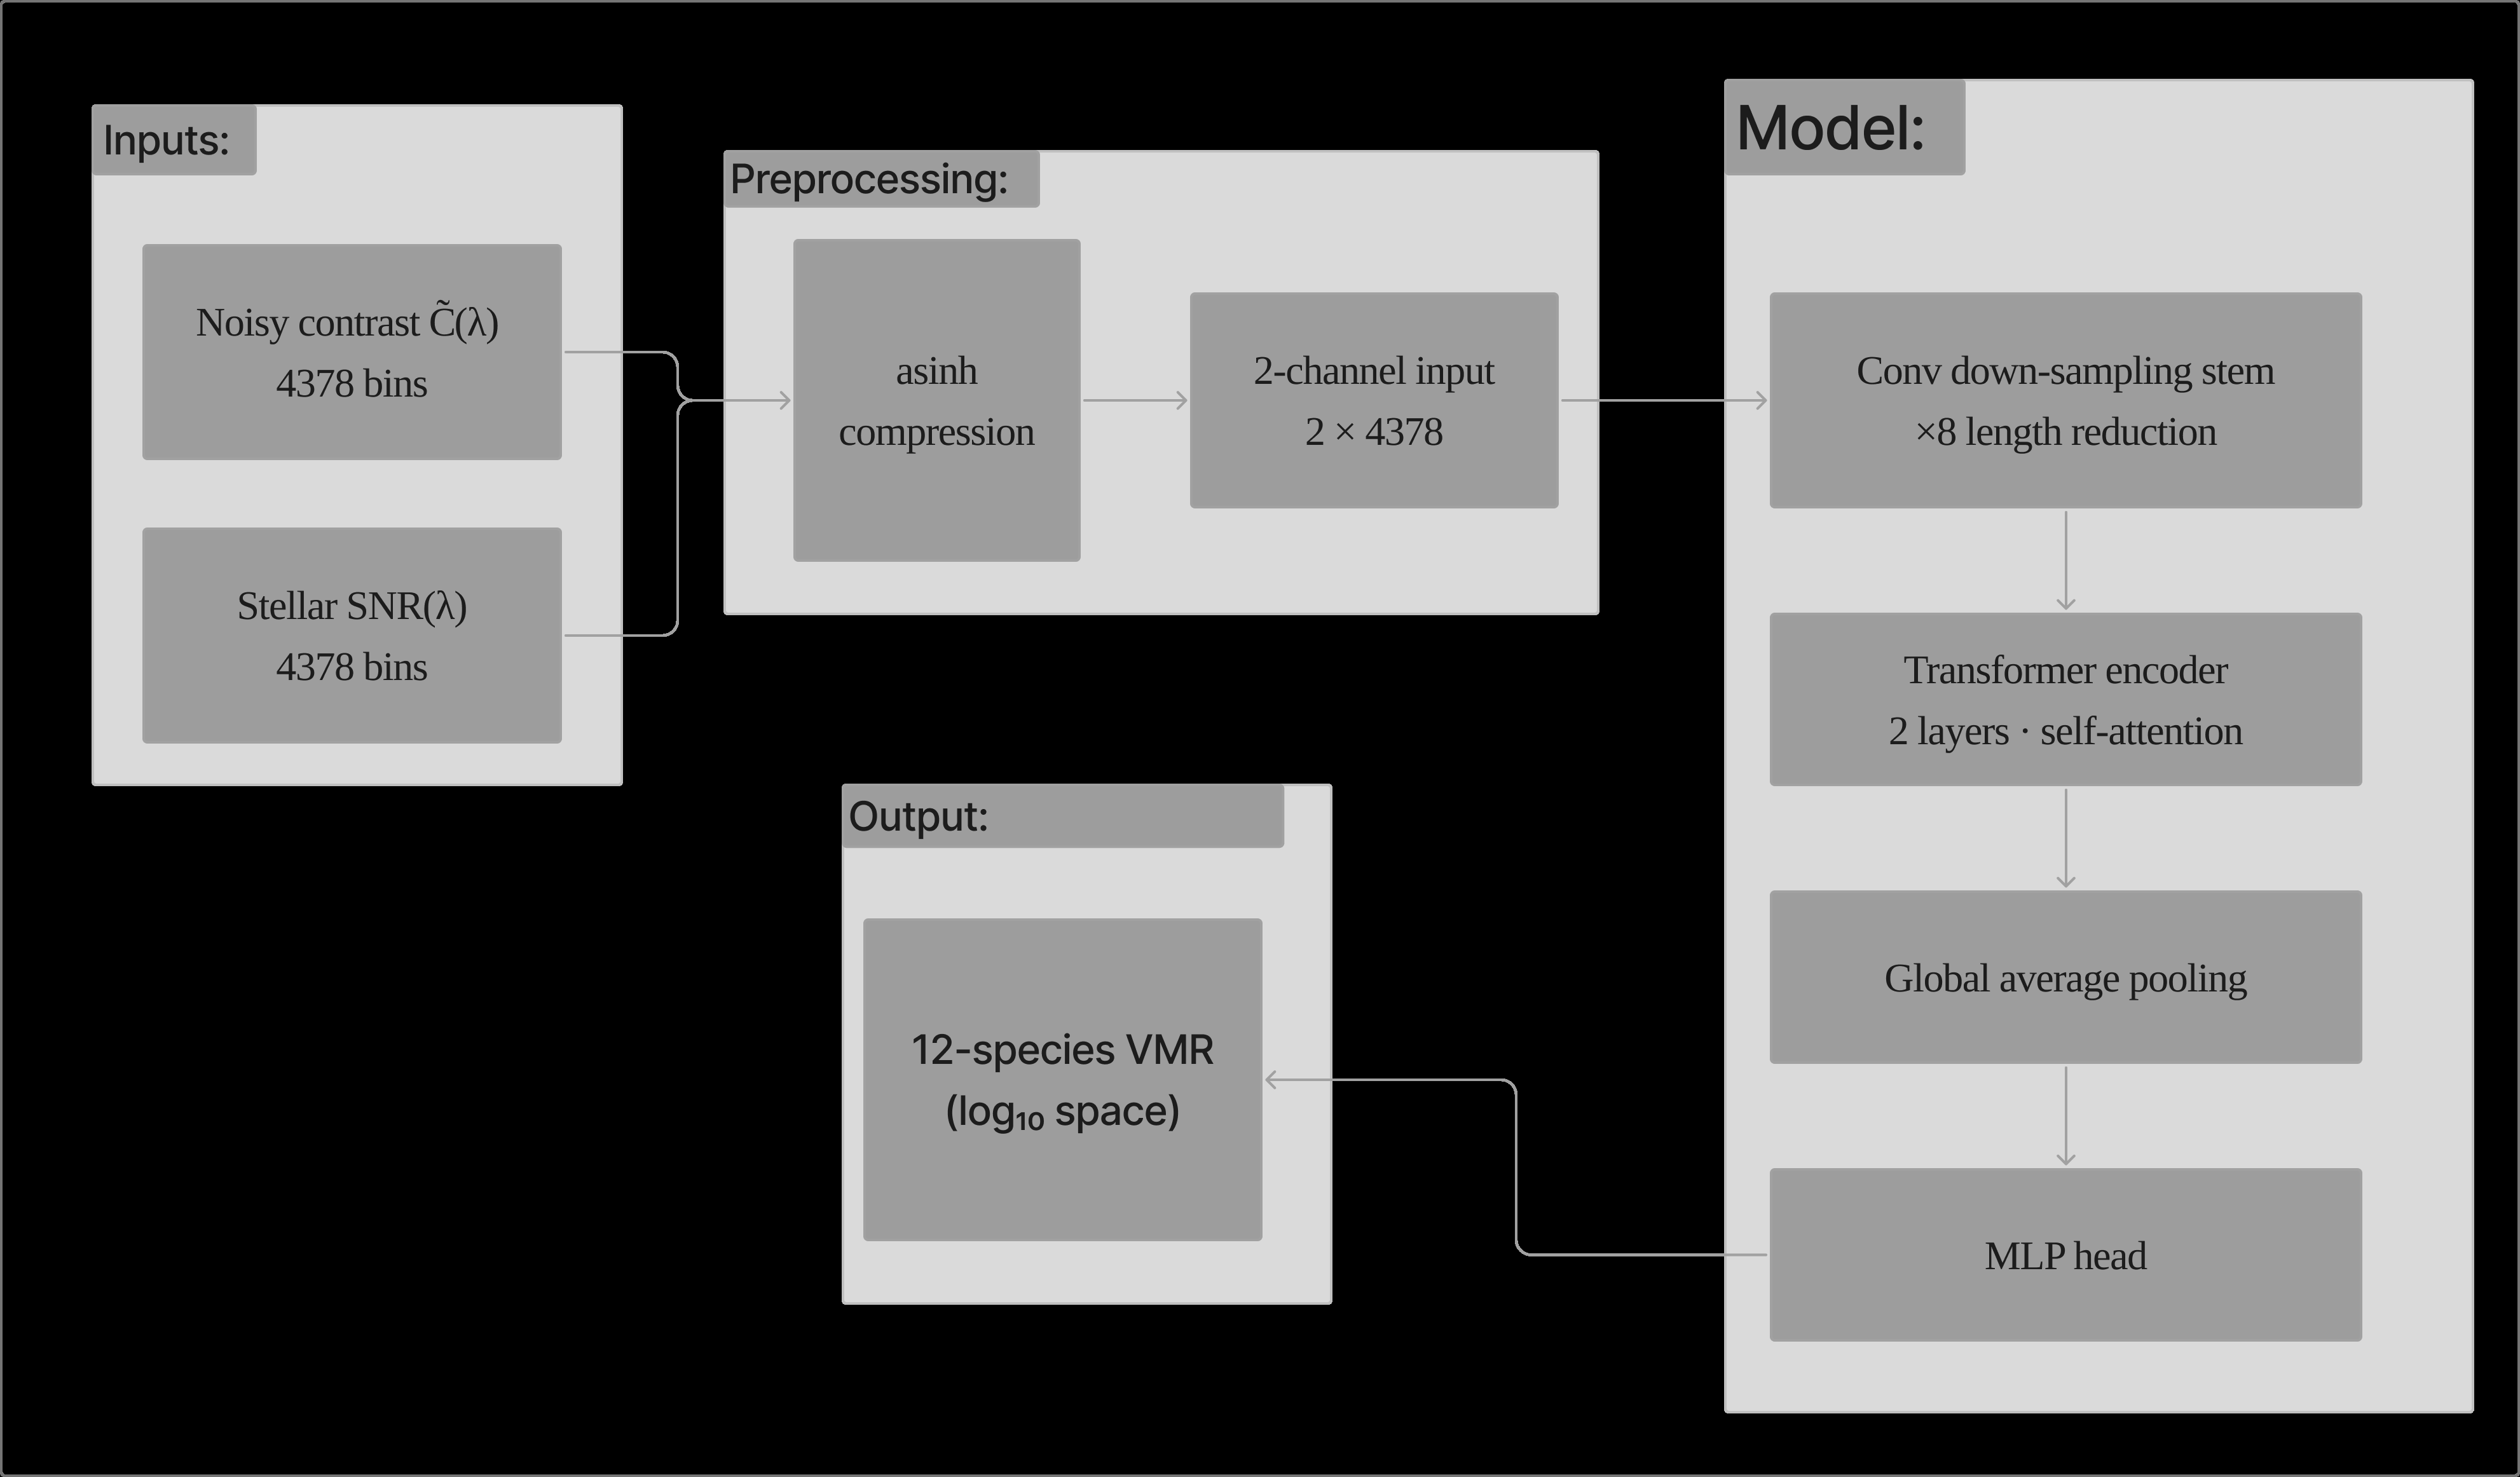
\includegraphics[width=\linewidth]{fig_transformer_arch.png}
\caption{Transformer backbone shared by the \texttt{transformerarch} and
\texttt{causal} tracks. The two-channel contrast/SNR input (each $4378$ bins) is
asinh-compressed, then passes through a convolutional down-sampling stem
($\times 8$ length reduction), a two-layer Transformer encoder, global average
pooling, and an MLP head that outputs the 12-species VMR vector.}
\label{fig:transdiag}
\end{figure}

\subsection{Counterfactual (causal) model}
\label{sec:causal}

Treat composition $a$ and observing environment $e$ (host star, distance, noise)
as independent causes of a spectrum $x=g(a,e)$. The atmosphere is the quantity of
interest; the environment is a nuisance that a reliable retrieval should ignore.
A counterfactual applies the intervention $\mathrm{do}(e{=}e_j)$, holding the
atmosphere of planet $i$ fixed while substituting the environment of planet $j$,
\begin{equation}
x_i^{\mathrm{do}(e=e_j)} = g(a_i,e_j),
\end{equation}
constructed by re-pairing the star-free albedo of $i$ with the stellar and noise
profile of $j$. Training penalises any change in prediction under this
intervention,
\begin{equation}
\mathcal{L}=\mathcal{L}_\mathrm{task}
+\lambda\,\big\lVert f(x_i)-f\!\big(x_i^{\mathrm{do}(e=e_j)}\big)\big\rVert^2 ,
\end{equation}
so the network is rewarded for invariance to the environment while retaining the
atmospheric signal (Figure~\ref{fig:causaldiag}). Because the counterfactual
re-pairs existing components rather than generating new ones, the augmentation
introduces no synthetic artefacts and cannot leak label information.

\begin{figure}[t]
\centering
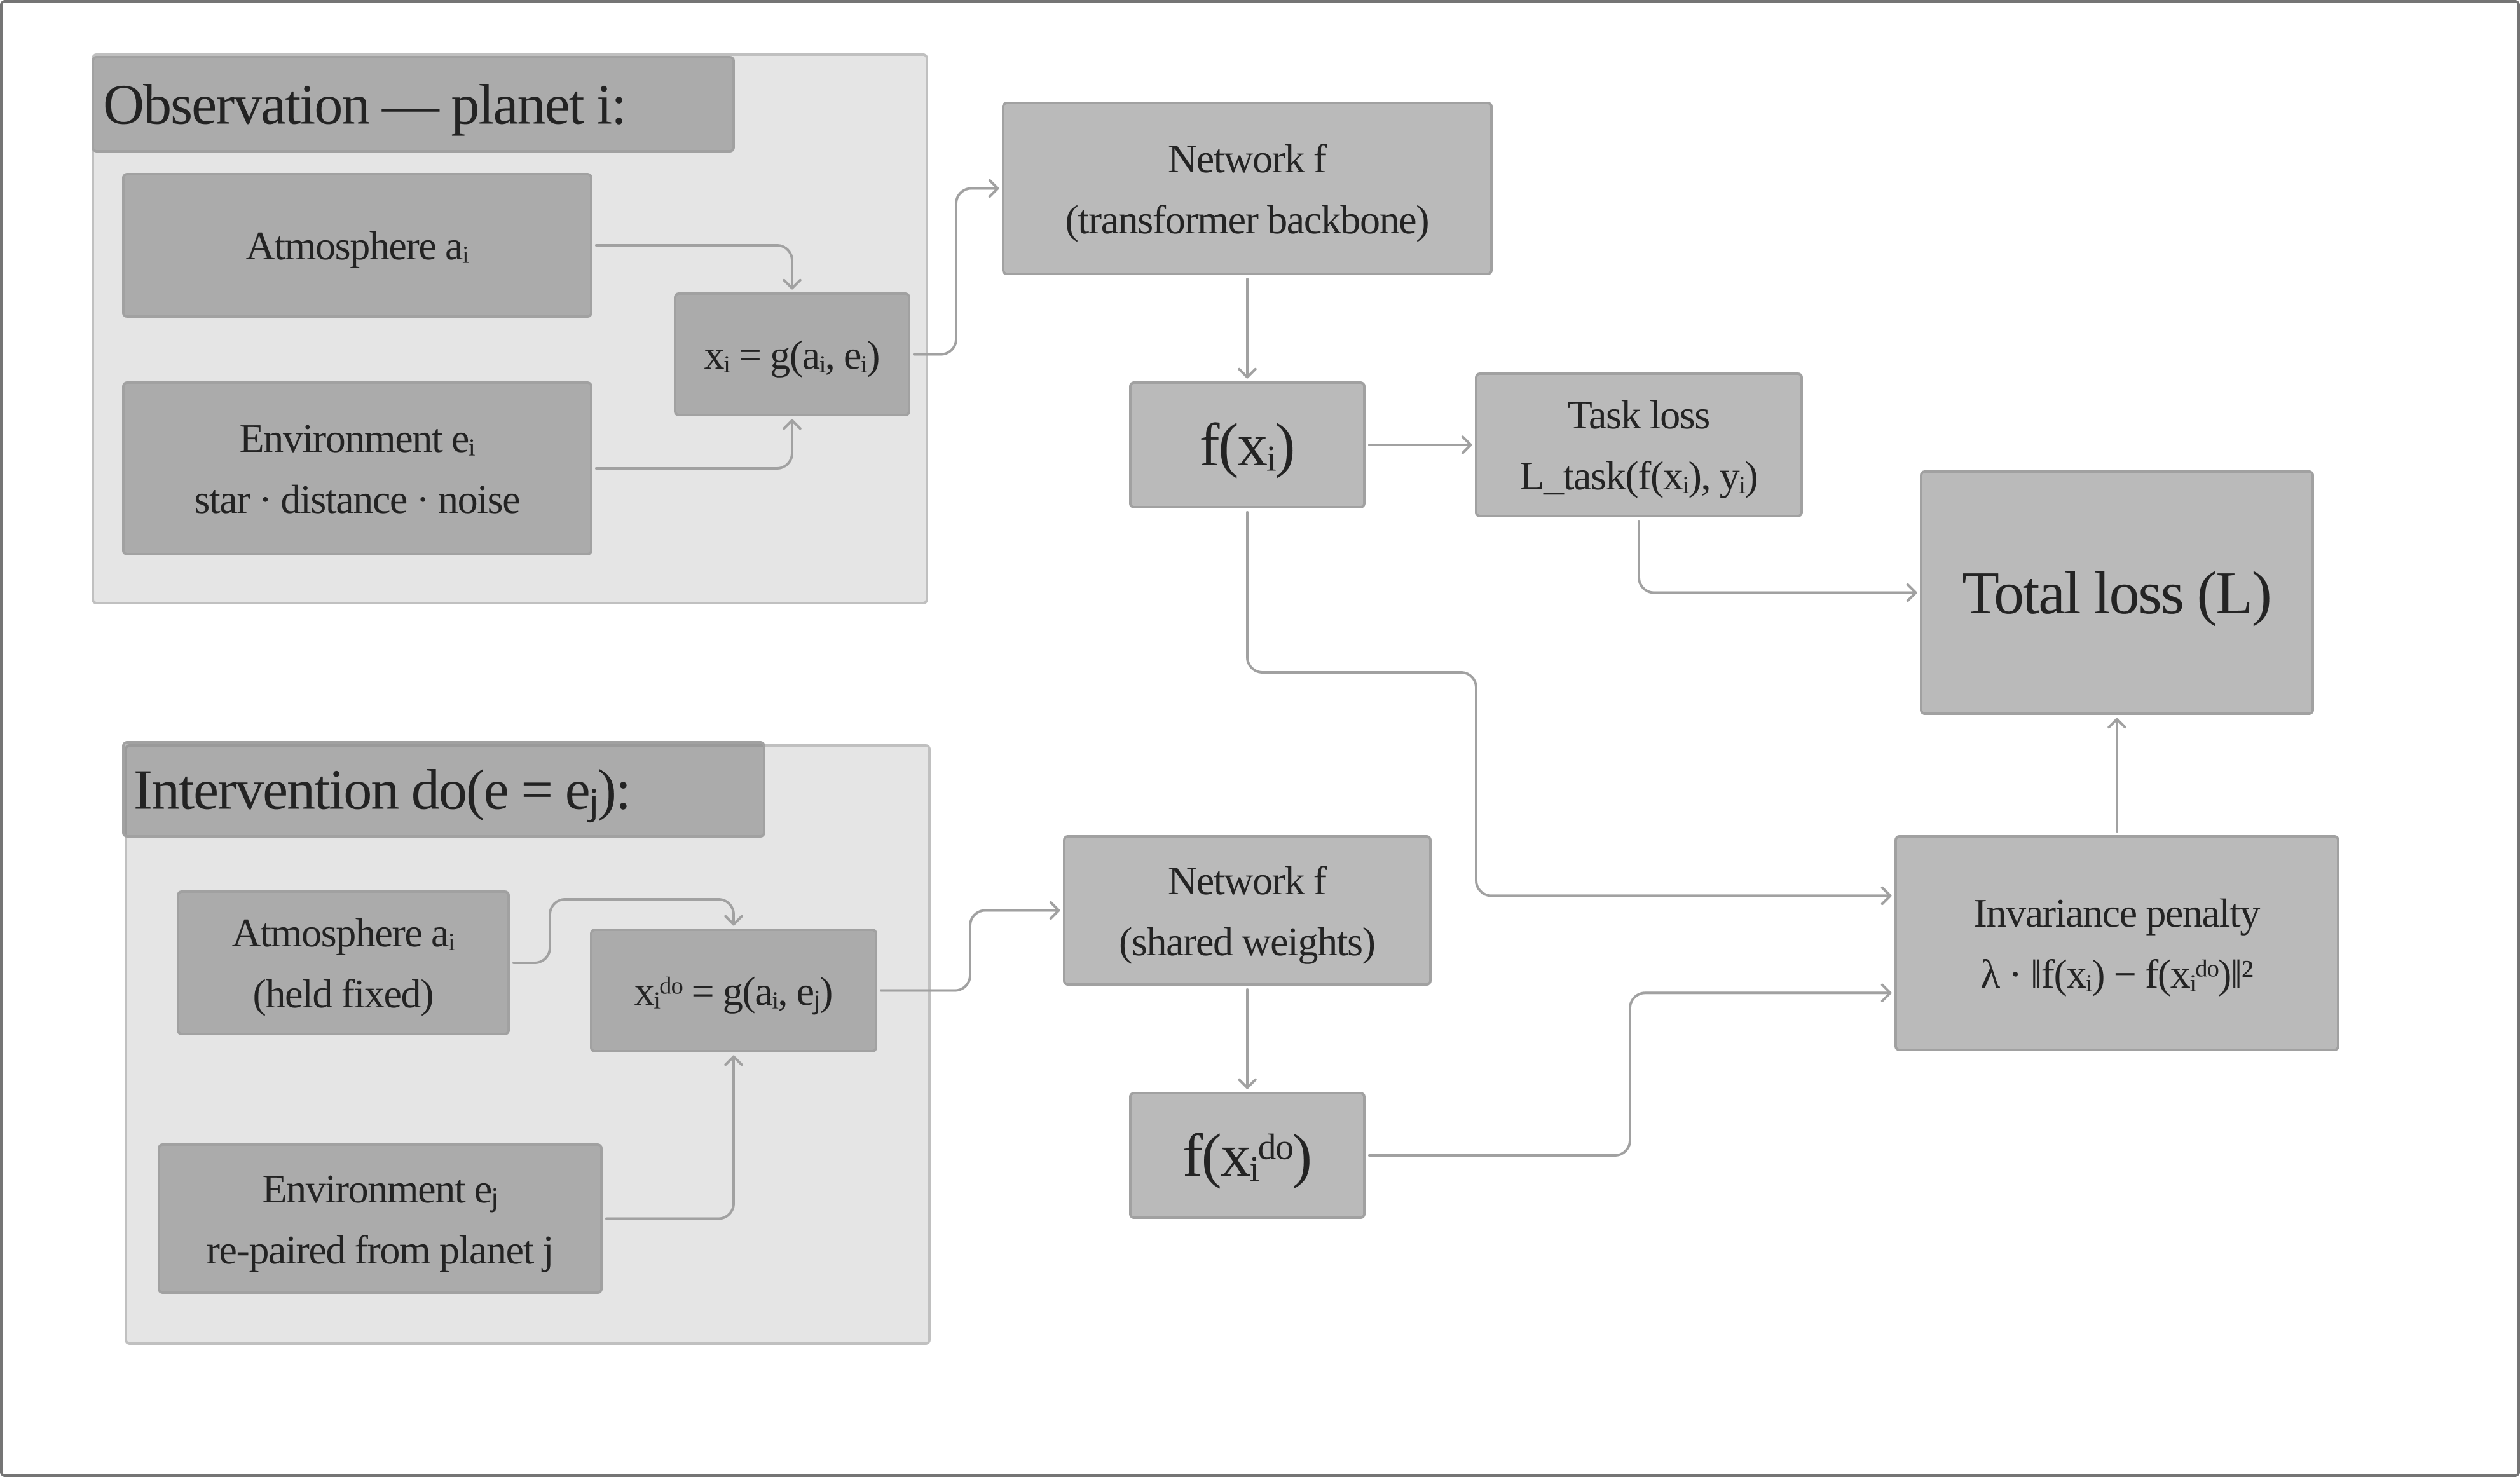
\includegraphics[width=\linewidth]{fig_causal_arch.png}
\caption{Counterfactual augmentation. The atmosphere of planet $i$ is re-paired
with the observing environment of planet $j$ to form an interventional spectrum,
and the shared network is penalised for any change in its prediction between the
two.}
\label{fig:causaldiag}
\end{figure}

\subsection{Classical and physics baselines}
\label{sec:baselines}

To gauge what the networks add, we include three simulator-agnostic baselines,
evaluated at $\alpha{=}1$ on the full 12-species target: a prior-mean predictor
(the training-set mean, ignoring the spectrum entirely), ridge regression, and a
random forest, the latter two on features formed by average-pooling each channel
to 64 wavelength bins. For the real-data methane test we also use a hand-built
band-depth ruler, a one-parameter physics statistic that measures absorption
depth in the \ch{} bands relative to the local continuum, with no learned
parameters. The ruler is a deliberately transparent yardstick: if a network
cannot beat it, the network has added nothing on that task.

\subsection{Inference-time bias correction}
\label{sec:corr_method}

Two corrections are applied to already-trained models, with no retraining. Let
$x$ be a spectrum and $x_c$ its continuum twin, obtained by low-pass filtering
away molecular absorption. The prior-driven offset is common to both, so
subtracting the twin prediction cancels the per-body baseline while preserving
the feature-driven response,
\begin{equation}
\hat{y}_\mathrm{null}=f(x)-f(x_c).
\end{equation}
Separately, we stack the frozen architectures through a per-species
ordinary-least-squares fit on one half of the synthetic validation set, scored on
the other. Because the architectures make different errors, the stack is more
stable than any single model.

\subsection{Neural de-clouding}
\label{sec:decloud_method}

Clouds mute atmospheric absorption and degrade retrieval. A separate network $d$
of about 1M parameters reconstructs a pseudo-clear spectrum from a cloudy one,
trained on grey (wavelength-independent) cloud pairs by
$\min_d\lVert d(x_\mathrm{cloudy})-x_\mathrm{clear}\rVert$ and evaluated on
held-out cloud morphologies (non-grey haze, band-selective, and Earth-like
patchy clouds). We report it as a negative result
(Section~\ref{sec:decloud_res}).

\subsection{Uncertainty and metrics}
\label{sec:uq_method}

We compare two uncertainty estimates: the spread of a small architecture
ensemble, and split-conformal prediction, which calibrates per-species intervals
on a held-out split to reach a target coverage by construction. Both are tested
under spectral-resolution shift, and we introduce a resolution-conditioned
conformal variant that recomputes quantiles at the target resolving power without
retraining. Retrieval accuracy is the coefficient of determination $R^2$ in
$\log_{10}$-VMR space, the space in which trace gases contribute proportionately;
we also report RMSE and MAE in dex. Detection on real data uses the area under
the ROC curve (AUROC) with 95\% bootstrap confidence intervals over the test
bodies. Every accuracy figure is quoted at the noiseless ceiling, at
$\alpha{=}1$, or both.

% ==================================================================
\section{Results}
% ==================================================================

\subsection{Accuracy, model size, and the causal ablation}
\label{sec:accuracy}

Accuracy does not increase with model size (Table~\ref{tab:arch},
Figure~\ref{fig:arch}). The 520k-parameter causal model reaches the highest
ceiling ($R^2{=}0.781$), level with the 36M-parameter convolutional baseline
($0.779$) despite being roughly $70\times$ smaller. What mattered was the input
representation (dimensionless contrast plus an SNR channel) and the
exposure-aware noise model, not the parameter count. On the identical
520k-parameter backbone, adding counterfactual augmentation raises the ceiling
from $0.568$ (\texttt{transformerarch}) to $0.781$ (\texttt{causal}), a gain of
$+0.213$ attributable to the training objective alone, since the two tracks share
architecture, budget, and data. Enlarging the causal backbone did not help
(\texttt{causal\_xl}, $0.173$), consistent with the compact model already
saturating the information available at this resolution.

Two caveats bound the ablation. It is measured at the noiseless ceiling and from
single-seed runs. At the realistic single exposure, all architectures collapse
toward a common photon-limited floor ($R^2\!\approx\!0.05$ to $0.13$), where the
ceiling gap is no longer resolvable, so the augmentation buys accuracy in the
high-signal regime rather than rescuing a photon-starved observation. A per-gas
linear stack of the six frozen models raises the ceiling to $0.849$
(Figure~\ref{fig:stack}), above both the best single model ($0.777$) and a naive
six-model mean ($0.637$). The apparent architecture ceiling near $0.78$ was
therefore complementary error across models, not an information limit of the
data.

\begin{table}[t]
\centering
\caption{Architecture comparison at the noiseless ceiling (covered-gas $R^2$,
$\log_{10}$-VMR). \texttt{causal} and \texttt{transformerarch} share the same
520k backbone and differ only in training objective.}
\label{tab:arch}
\small
\begin{tabular}{@{}lrrc@{}}
\toprule
Model & Params & Ceiling & $\alpha{=}1$ \\
\midrule
\texttt{causal}          & 0.52M & 0.781 & 0.128 \\
\texttt{original1dcnn}   & 36M   & 0.779 & -- \\
\texttt{optimized1dcnn}  & 1.2M  & 0.728 & -- \\
\texttt{transformerarch} & 0.52M & 0.568 & -- \\
\texttt{causal\_xl}      & 2M    & 0.173 & -- \\
\midrule
Per-gas stack (6 models) & --    & 0.849 & -- \\
\bottomrule
\end{tabular}
\end{table}

\begin{figure}[t]
\centering
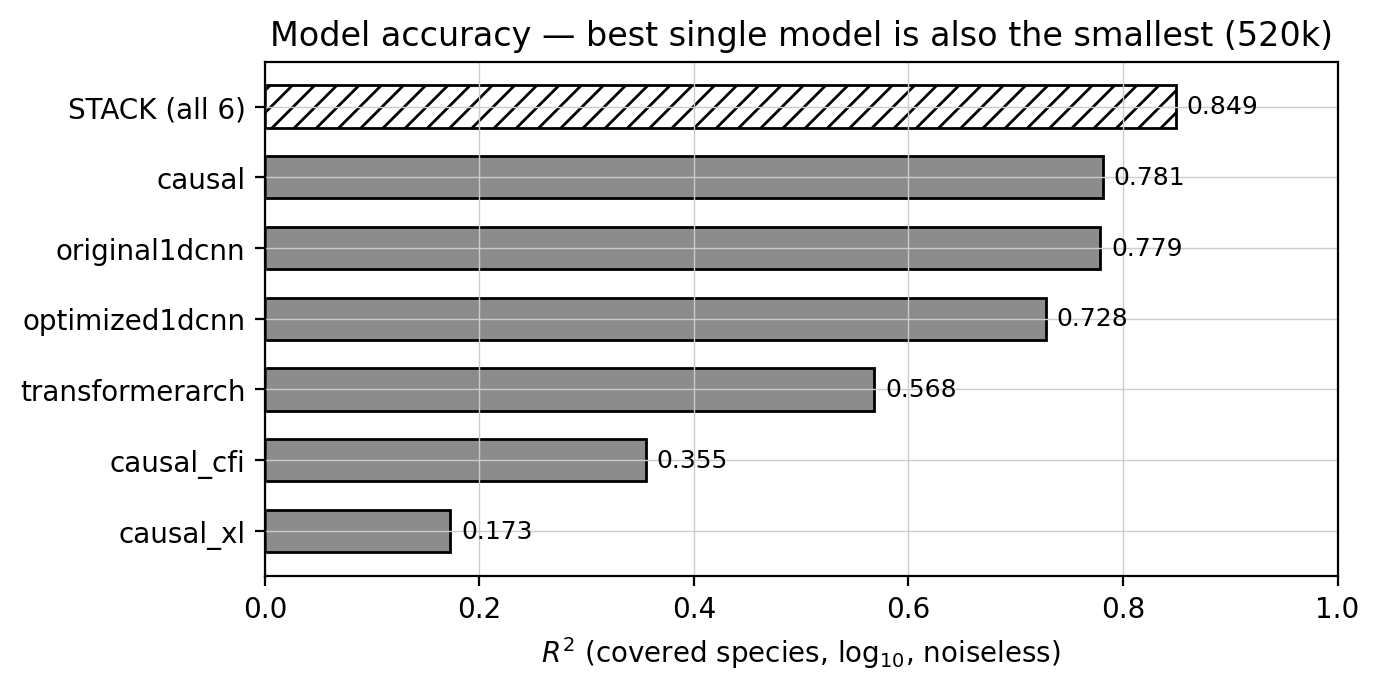
\includegraphics[width=\linewidth]{fig01_model_accuracy.png}
\caption{Accuracy across architectures at the noiseless ceiling: flat with
respect to model size, with the compact causal model matching the 36M-parameter
baseline.}
\label{fig:arch}
\end{figure}

\begin{figure}[t]
\centering
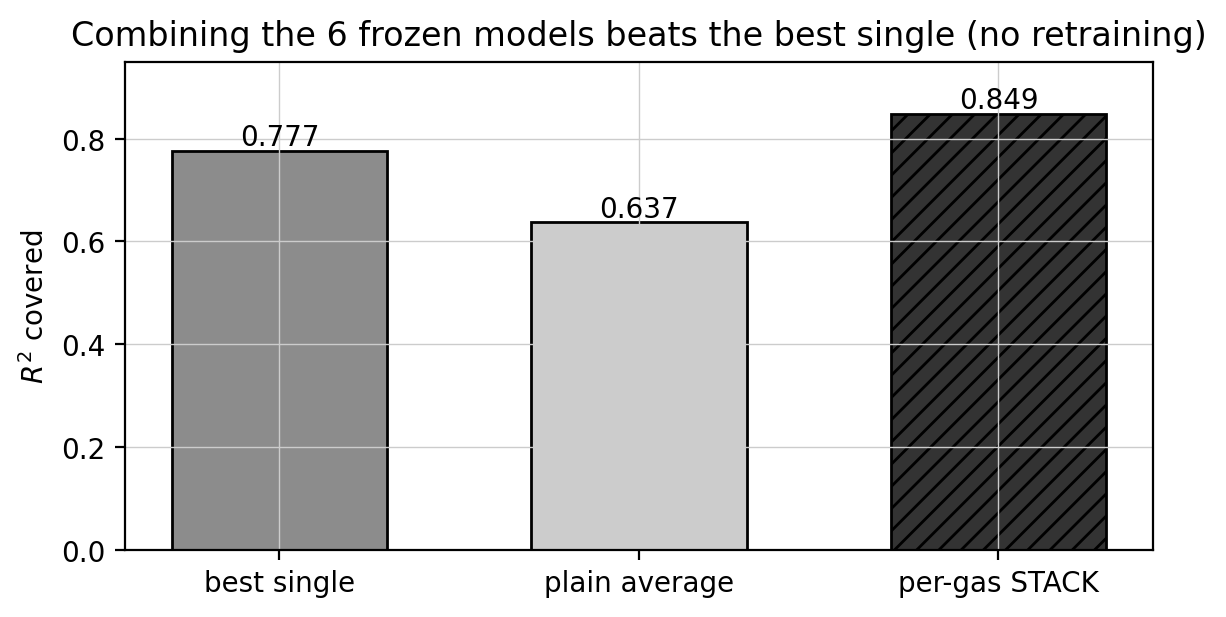
\includegraphics[width=\linewidth]{fig12_model_stacking.png}
\caption{Per-gas linear stacking of frozen models beats the best single model and
a naive average, indicating the ceiling was complementary error.}
\label{fig:stack}
\end{figure}

\subsection{Exposure time and per-gas accuracy}
\label{sec:exposure}

Retrieval is photon-limited across the entire practical range
(Table~\ref{tab:exposure}, Figure~\ref{fig:exposure}). At the realistic single
exposure the covered-gas $R^2$ is only $0.13$, and the $0.78$ ceiling is
approached only near $10^4\times$ nominal exposure, far beyond any feasible
integration. This is the clearest single illustration of the paper's theme: the
number that looks impressive (the ceiling) and the number that describes a real
observation ($\alpha{=}1$) differ by a factor of six, and only the latter
predicts what a telescope would return.

Per-gas behaviour shows the same split (Table~\ref{tab:pergas},
Figure~\ref{fig:pergas}). Ceilings of $0.72$ to $0.86$ for the covered gases fall
to $0.03$ to $0.33$ at $\alpha{=}1$, with ozone the most resilient because its
broad Chappuis band survives noise better than narrow features. Nitrogen has no
reflected-light features, so no model retrieves it; its $R^2$ is negative at both
operating points ($\approx-0.06$), and we report that value rather than omit it,
since an honest null is itself informative. The derived carbon-to-oxygen (C/O)
ratio, an indicator of formation history, reaches $R^2{=}0.81$ at the ceiling
(median error $0.05$\,dex) but falls to $0.10$ at $\alpha{=}1$, so a quantity
often quoted as a headline product is essentially unconstrained at realistic
exposure. Temperature and metallicity are not retrieval targets of the INARA data
set and are not reported.

\begin{table}[t]
\centering
\caption{Covered-gas $R^2$ (causal) versus exposure factor. $\alpha{=}1$ is the
realistic single exposure; the ceiling is reached only at extreme integration.}
\label{tab:exposure}
\small
\setlength{\tabcolsep}{4pt}
\begin{tabular}{@{}lccccccc@{}}
\toprule
$t_\mathrm{exp}/t_\mathrm{nom}$ & 0.09 & 1 & 9 & 100 & 900 & $10^4$ & $9{\times}10^4$ \\
\midrule
$R^2$ & $-0.02$ & 0.13 & 0.35 & 0.56 & 0.70 & 0.79 & 0.83 \\
\bottomrule
\end{tabular}
\end{table}

\begin{figure}[t]
\centering
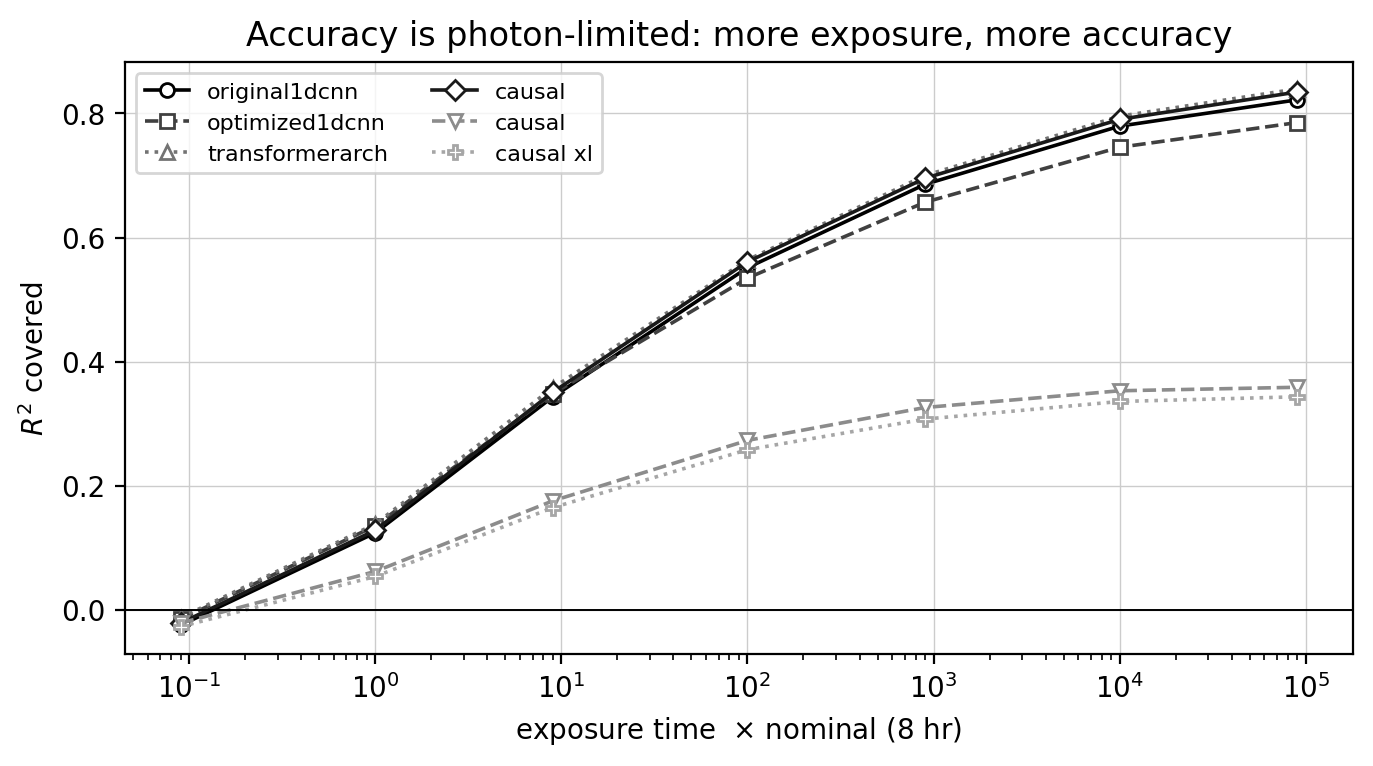
\includegraphics[width=\linewidth]{fig04_exposure_accuracy.png}
\caption{Accuracy versus exposure time: set by the photon budget rather than by
the model across the practical range.}
\label{fig:exposure}
\end{figure}

\begin{table}[t]
\centering
\caption{Per-gas accuracy (causal) at the noiseless ceiling and at $\alpha{=}1$,
with realistic-exposure RMSE. \ntwo{} is spectrally invisible in this band.}
\label{tab:pergas}
\small
\begin{tabular}{@{}lccc@{}}
\toprule
Gas & Ceiling & $\alpha{=}1$ & RMSE $\alpha{=}1$ (dex) \\
\midrule
\wat & 0.72 & 0.06 & 0.44 \\
\co  & 0.73 & 0.03 & 0.36 \\
\ot  & 0.80 & 0.12 & 0.36 \\
\ch  & 0.79 & 0.11 & 0.42 \\
\oth & 0.86 & 0.33 & 0.48 \\
\ntwo & $-0.06$ & $-0.06$ & -- \\
\bottomrule
\end{tabular}
\end{table}

\begin{figure}[t]
\centering
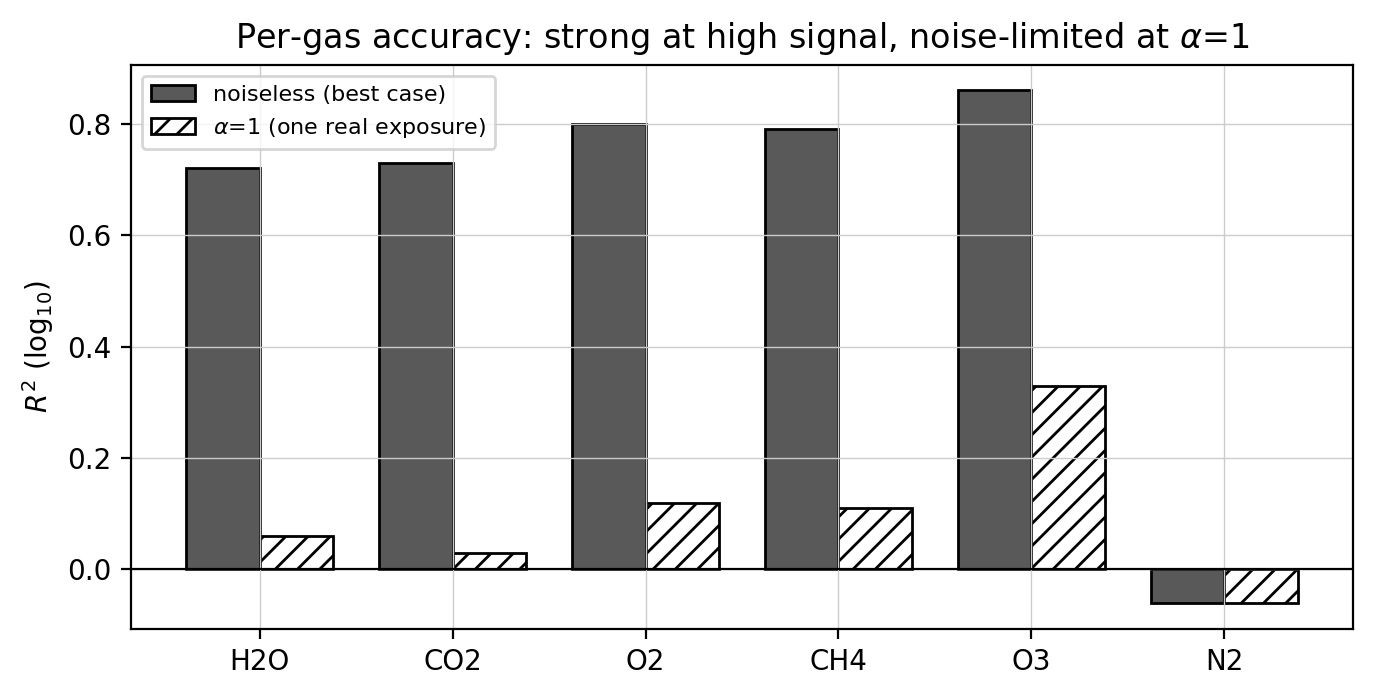
\includegraphics[width=\linewidth]{fig03_pergas_accuracy.png}
\caption{Per-gas accuracy at the two operating points. Ozone is the most
exposure-robust species; nitrogen is unretrievable by construction.}
\label{fig:pergas}
\end{figure}

\subsection{Classical baselines}
\label{sec:baselines_res}

At the realistic single exposure the simulator-agnostic baselines set the bar the
networks must clear (Table~\ref{tab:baselines}, Figure~\ref{fig:baselines}). The
prior-mean predictor scores $R^2{=}-0.06$ on the 12-species target, so predicting
the training mean alone carries no skill. Ridge regression and a random forest
reach $0.03$ and $0.01$. The neural model reaches $0.13$ on covered gases at the
same $\alpha{=}1$, a genuine improvement over the classical methods, but a small
absolute number that underlines how little quantitative information survives
realistic photon noise. The gap between this and the ceiling is not a modelling
deficiency to be engineered away; it is the photon budget.

\begin{table}[t]
\centering
\caption{Classical baselines at $\alpha{=}1$ (12-species overall $R^2$,
$\log_{10}$-VMR). The neural model reaches $0.13$ on covered gases at the same
exposure.}
\label{tab:baselines}
\small
\begin{tabular}{@{}lccc@{}}
\toprule
Baseline & $R^2$ & RMSE (dex) & MAE (dex) \\
\midrule
Prior mean    & $-0.059$ & 0.474 & 0.325 \\
Ridge         & $0.031$  & 0.452 & 0.312 \\
Random forest & $0.013$  & 0.456 & 0.314 \\
\bottomrule
\end{tabular}
\end{table}

\begin{figure}[t]
\centering
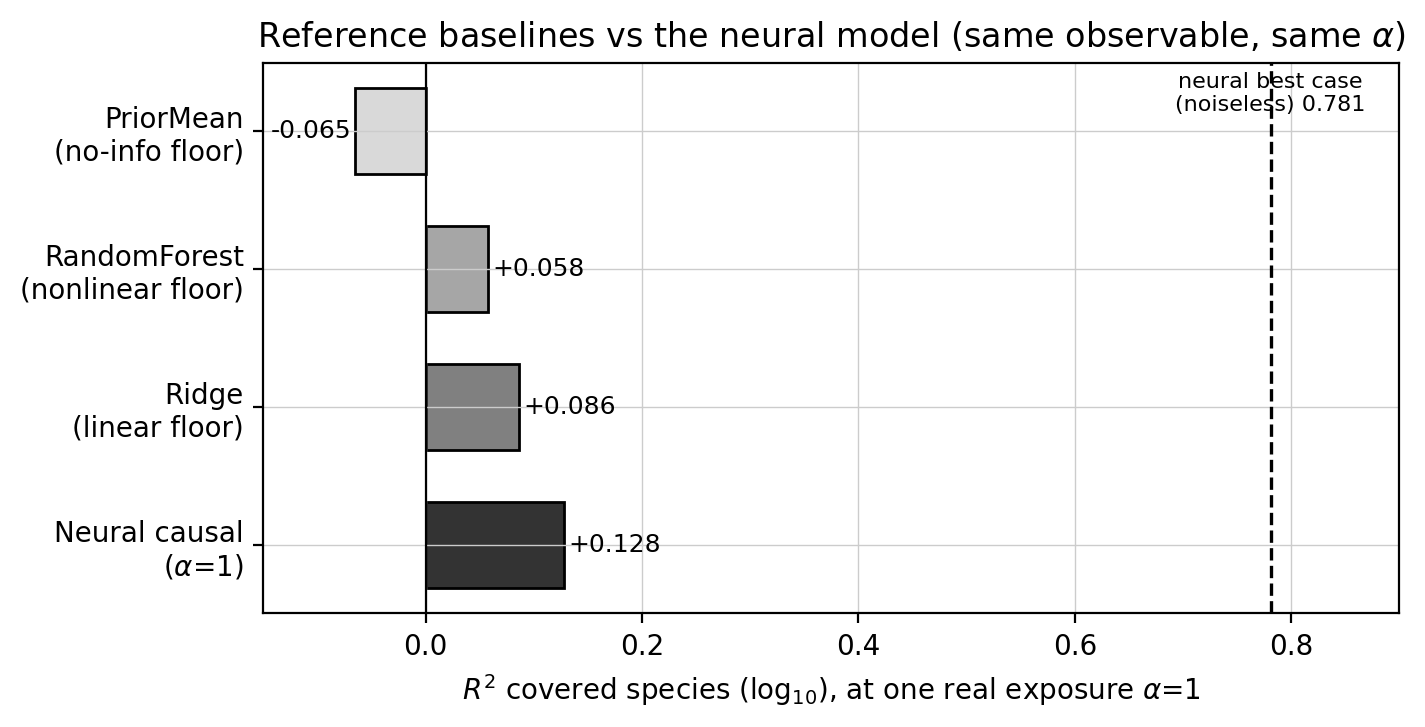
\includegraphics[width=\linewidth]{fig13_baselines.png}
\caption{Neural retrieval versus classical baselines at $\alpha{=}1$. The network
adds value over ridge and random forest, but all three sit far below the ceiling.}
\label{fig:baselines}
\end{figure}

\subsection{Spectral resolution}
\label{sec:resolution}

Resolving power controls which gases are retrievable at all
(Table~\ref{tab:resolution}, Figure~\ref{fig:resolution}). Ozone retains
$R^2{=}0.80$ down to $R{=}22$, whereas \co{} degrades sharply below $R{=}200$ and
cannot be recovered at $R{=}22$ even with affine recalibration: at that
resolution the information is destroyed, not merely miscalibrated, and no
post-hoc correction can restore it. Most other gases become recalibratable from
about $R{=}50$. This has a direct real-data consequence. Venus and Mars are
observed at $R\!\approx\!22$ in the catalogue, so their retrieval failure is
imposed by physics rather than by the model, and it would be a mistake to read
their poor numbers as evidence about the network.

\begin{table*}[t]
\centering
\caption{Per-gas $R^2$ versus resolving power (causal), reported as raw\,/\,affine-recalibrated. \co{} is unrecoverable at $R{=}22$; \oth{} survives to the lowest resolution tested.}
\label{tab:resolution}
\small
\begin{tabular}{@{}lccccc@{}}
\toprule
$R$ & \wat & \co & \ot & \ch & \oth \\
\midrule
22     & $-0.24$\,/\,$0.36$ & $-1.87$\,/\,$0.11$ & $-0.15$\,/\,$0.33$ & $0.32$\,/\,$0.34$ & $0.27$\,/\,$0.80$ \\
50     & $0.48$\,/\,$0.54$  & $-4.37$\,/\,$0.09$ & $0.26$\,/\,$0.53$  & $0.50$\,/\,$0.56$ & $0.55$\,/\,$0.85$ \\
100    & $0.55$\,/\,$0.61$  & $-1.82$\,/\,$0.22$ & $0.53$\,/\,$0.69$  & $0.64$\,/\,$0.68$ & $0.67$\,/\,$0.87$ \\
200    & $0.64$\,/\,$0.67$  & $0.39$\,/\,$0.52$  & $0.71$\,/\,$0.76$  & $0.74$\,/\,$0.76$ & $0.76$\,/\,$0.88$ \\
400    & $0.60$\,/\,$0.68$  & $0.68$\,/\,$0.68$  & $0.78$\,/\,$0.78$  & $0.79$\,/\,$0.81$ & $0.81$\,/\,$0.89$ \\
870    & $0.59$\,/\,$0.70$  & $0.70$\,/\,$0.70$  & $0.80$\,/\,$0.79$  & $0.80$\,/\,$0.82$ & $0.83$\,/\,$0.89$ \\
native & $0.71$\,/\,$0.74$  & $0.74$\,/\,$0.74$  & $0.80$\,/\,$0.84$  & $0.78$\,/\,$0.83$ & $0.83$\,/\,$0.89$ \\
\bottomrule
\end{tabular}
\end{table*}

\begin{figure}[t]
\centering
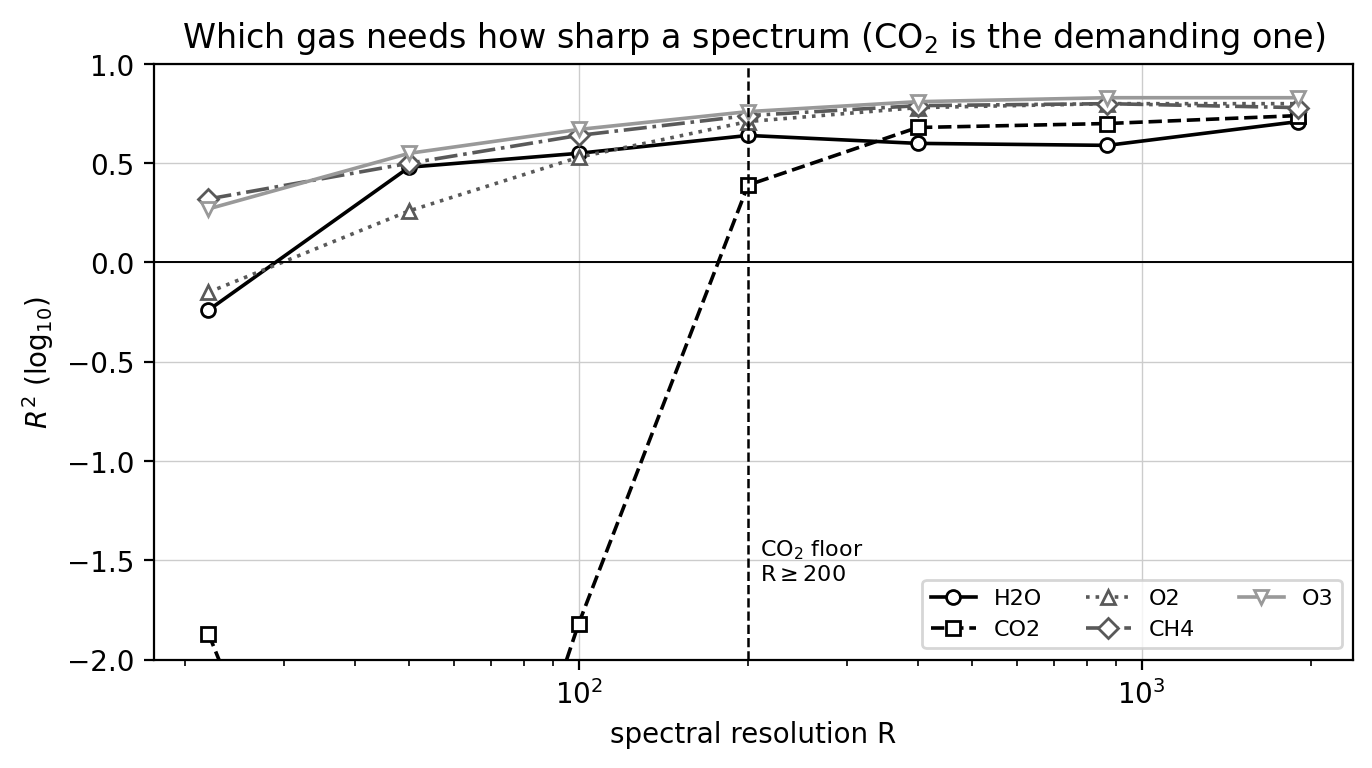
\includegraphics[width=\linewidth]{fig10_resolution_requirements.png}
\caption{Accuracy versus resolving power. \co{} needs $R\!\ge\!200$; \oth{}
remains usable to $R{=}22$.}
\label{fig:resolution}
\end{figure}

\subsection{Cross-simulator generalisation}
\label{sec:crosssim}

Applied without adaptation to spectra from a different forward model, every model
loses accuracy (Table~\ref{tab:crosssim}, Figure~\ref{fig:crosssim}). This is
expected. pRT and TauREx use different radiative-transfer engines and target
regimes, and TauREx in particular is tuned for gaseous giants rather than the
rocky atmospheres of INARA, so their spectral statistics differ from PSG. An
attempt to train jointly across two such sets did not produce a shared
improvement, because the differences are in the generators rather than in the
underlying physics of any one planet. Adaptive Batch Normalisation, which
re-estimates normalisation statistics on unlabelled target spectra with no
retraining, removes most of the gap, and a light affine calibration brings it
close to zero, which points to covariate shift rather than lost information.
Among the models the causal track was the least affected. We do not read the
near-zero adapted values as positive transfer; they represent graceful recovery,
and cross-simulator generalisation remains an open problem.

\begin{table*}[t]
\centering
\caption{Cross-simulator covered-gas $R^2$ (noiseless reference). Adaptive Batch
Normalisation and a light affine calibration remove most of the collapse on pRT,
which points to covariate shift rather than an irreducible physics difference.}
\label{tab:crosssim}
\small
\begin{tabular}{@{}lccccc@{}}
\toprule
Model & PSG (native) & TauREx & pRT & pRT\,+\,AdaBN & pRT\,+\,affine \\
\midrule
\texttt{causal}         & 0.781 & $-0.33$ & $-3.05$ & -- & $\sim$0 \\
\texttt{optimized1dcnn} & 0.728 & $-0.27$ & $-3.74$ & $-0.16$ & $-0.04$ \\
\texttt{original1dcnn}  & 0.779 & $-0.37$ & $-5.56$ & -- & $-0.03$ \\
\bottomrule
\end{tabular}
\end{table*}

\begin{figure}[t]
\centering
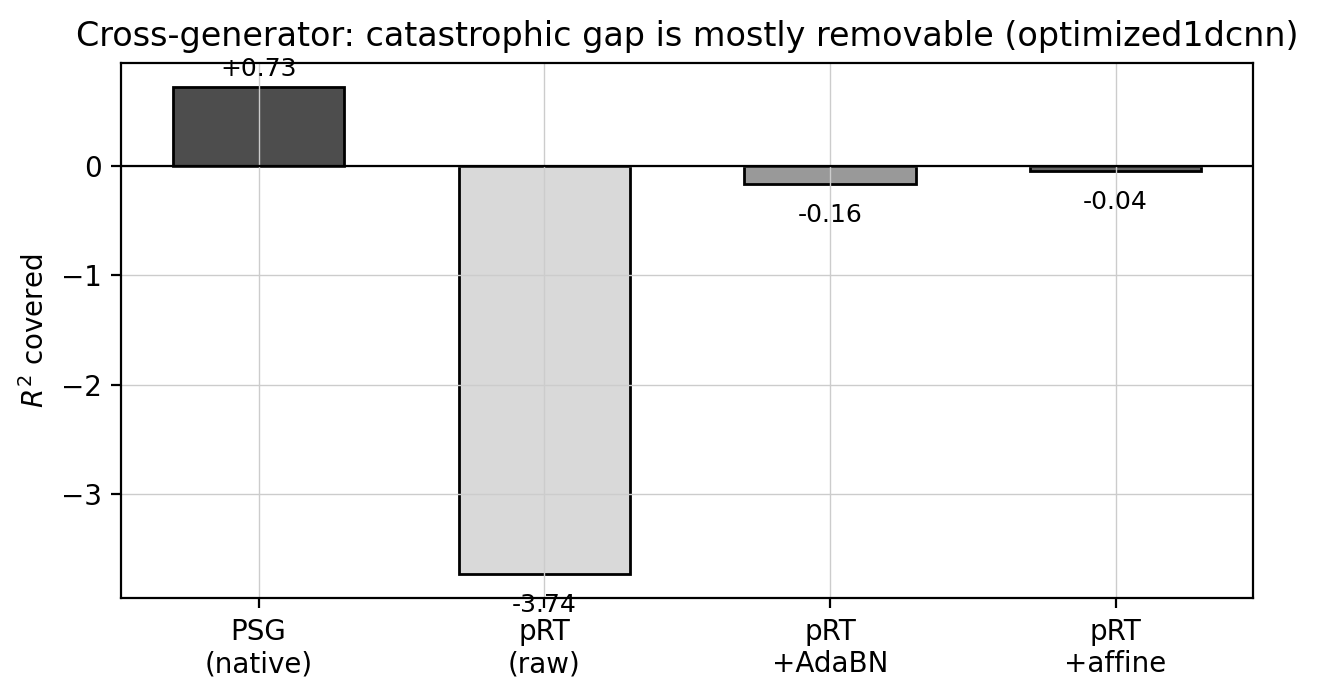
\includegraphics[width=\linewidth]{fig02_crossgen_adaptation.png}
\caption{Cross-simulator accuracy before and after Adaptive Batch Normalisation.
Most of the collapse is removable covariate shift.}
\label{fig:crosssim}
\end{figure}

\subsection{Predictive uncertainty}
\label{sec:uq}

Uncertainty estimates from the architecture ensemble are badly overconfident:
empirical 68\% coverage ranges from $0.08$ to $0.36$ against a $0.68$ target, so
the ensemble spread cannot be trusted as an error bar. Split-conformal intervals
are valid in-distribution (coverage $0.67$ to $0.71$, widths $0.13$ to
$0.20$\,dex), and these are the estimate we recommend. Both, however, break under
resolution shift: at $R{=}22$ the nominal intervals collapse to $0.16$ to $0.41$
coverage, which the resolution-conditioned conformal variant repairs by widening
the intervals appropriately (for \co, from $0.15$ to $0.58$\,dex) with no
retraining (Table~\ref{tab:uq}, Figure~\ref{fig:uq}). The lesson generalises: an
uncertainty estimate is reliable only within the distribution on which it was
calibrated, and a calibrated interval on synthetic data does not automatically
transfer to a real observation at a different resolution.

\begin{table}[t]
\centering
\caption{Per-gas conformal intervals (causal): native width and 68\% coverage,
coverage under an uncorrected $R{=}22$ shift, and the width required for correct
coverage there.}
\label{tab:uq}
\small
\setlength{\tabcolsep}{4pt}
\begin{tabular}{@{}lcccc@{}}
\toprule
Gas & Width & Cov nat. & Cov $R{=}22$ & Req.\ width \\
\midrule
\wat & 0.20 & 0.71 & 0.36 & 0.45 \\
\co  & 0.15 & 0.71 & 0.20 & 0.58 \\
\ot  & 0.13 & 0.67 & 0.26 & 0.37 \\
\ch  & 0.16 & 0.67 & 0.41 & 0.32 \\
\oth & 0.18 & 0.67 & 0.16 & 0.57 \\
\bottomrule
\end{tabular}
\end{table}

\begin{figure}[t]
\centering
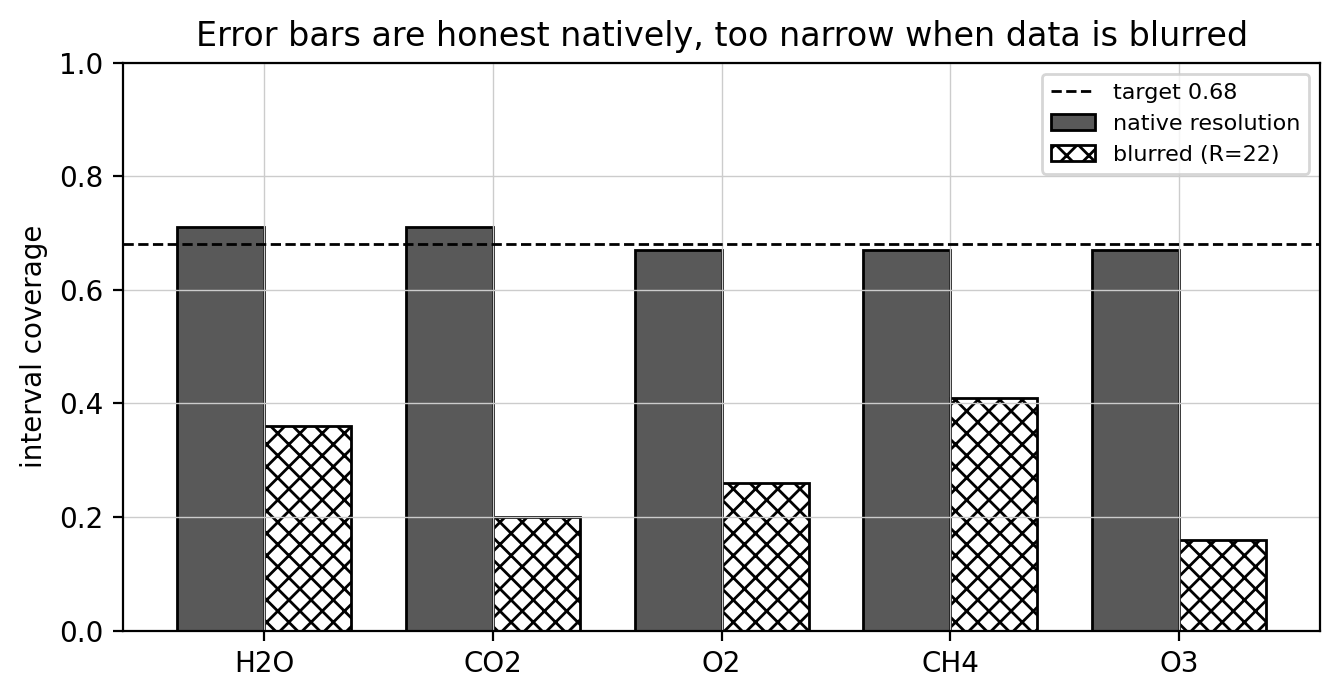
\includegraphics[width=\linewidth]{fig06_uncertainty_coverage.png}
\caption{Coverage of predictive intervals. The ensemble is overconfident;
split-conformal is calibrated in-distribution but must be resolution-conditioned
under shift.}
\label{fig:uq}
\end{figure}

\subsection{Comparison with Bayesian retrieval}
\label{sec:bayes}

The motivation for learned retrieval is cost, so the relevant baseline is
Bayesian inference. A nested-sampling retrieval of a single spectrum typically
requires \num{20000} to \num{60000} forward-model evaluations and hours of
wall-clock time \citep{ardevol2022,nixon2020}, whereas the neural models here
return a retrieval in a single sub-second forward pass, a speed-up of several
orders of magnitude. The price of that speed is reliability. The network's
accuracy is bounded by its training distribution, and it fabricates oxygen on
out-of-distribution inputs (Section~\ref{sec:realdata}) in a way a physics-based
retrieval, which evaluates a forward model against the actual data, would not.
Our findings are consistent with the literature on accuracy and calibration:
Nixon \& Madhusudhan \citep{nixon2020} report that supervised models match
nested-sampling estimates given enough training data, and M\'arquez-Neila et al.\
\citep{marquez2018} obtain posteriors consistent with Bayesian retrieval but
under-dispersed, the same under-dispersion we see in our ensemble and remedy with
conformal intervals. A full nested-sampling retrieval on the same real spectra,
matched to our forward model, is the natural next step and is beyond the present
scope.

\subsection{Real Solar-System spectra}
\label{sec:realdata}

\paragraph{Methane detection succeeds.} At matched resolution across bodies, four
of the six architectures achieve $\mathrm{AUROC}{=}1.00$ (95\% bootstrap CI
$[1.00,1.00]$) for separating methane-bearing atmospheres, such as Titan's, from
airless bodies; the remaining two score $0.88$ and $0.76$
(Figure~\ref{fig:ch4}). Two controls establish that this reflects genuine
spectral evidence. First, an occlusion test: blanking the \ch{} absorption bands
drops the AUROC to $0.88$, whereas blanking equally wide control bands leaves it
at $1.00$, so the models are reading methane rather than an incidental
correlate. Second, the hand-built band-depth ruler also scores $1.00$, so the
networks match, but do not exceed, a transparent one-parameter physics statistic
on this task. One caveat is statistical: the positive class contains few bodies,
so an AUROC of $1.00$ certifies clean separation on this sample rather than a
tight population estimate.

\begin{figure}[t]
\centering
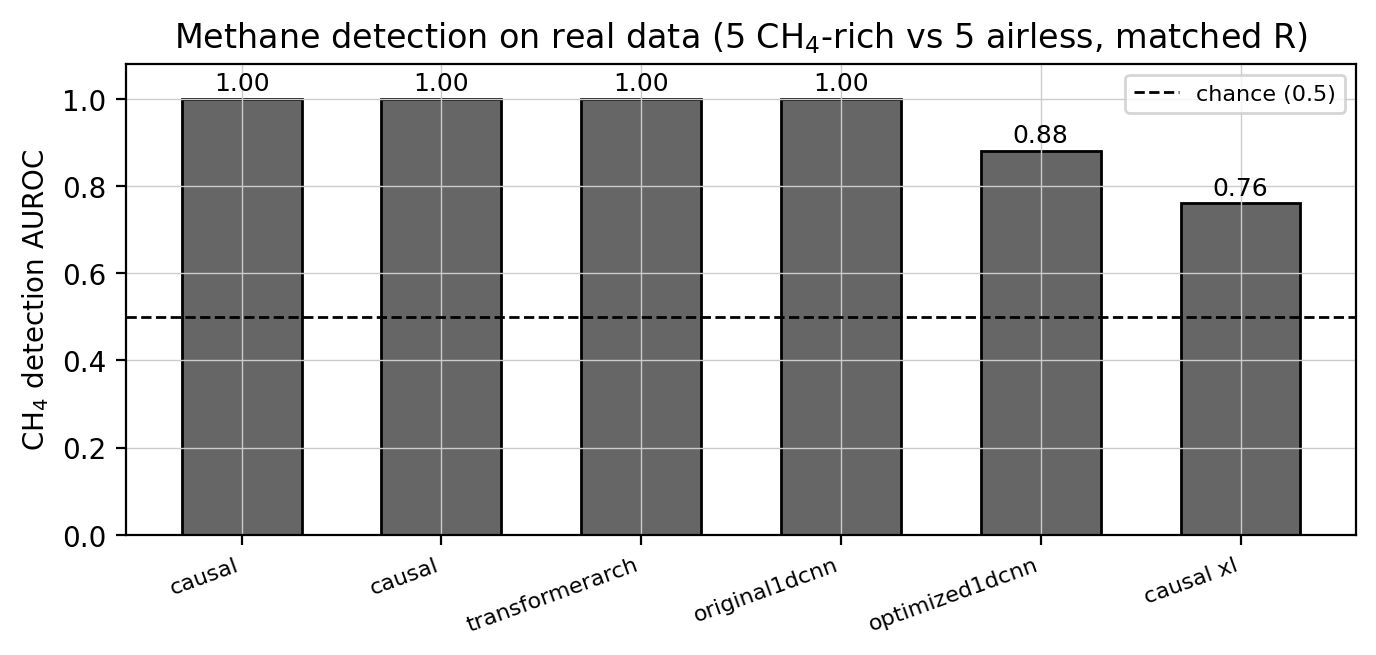
\includegraphics[width=\linewidth]{fig07_ch4_detection_auroc.png}
\caption{Methane detection on real spectra at matched resolution. Four of six
models, together with a physics ruler, separate methane-bearing from airless
bodies perfectly.}
\label{fig:ch4}
\end{figure}

\paragraph{Oxygen detection fails.} Every model assigns substantial oxygen (about
30 to 46\% predicted VMR) to airless bodies. In the cleanest test, the matched
Earth/Moon pair observed on the same night with the same instrument at the same
resolution, five of six models give the airless Moon \emph{more} oxygen than
Earth (Table~\ref{tab:earthmoon}), inverting the one contrast that matters for a
biosignature. The cause is not architecture but the training label prior: the
INARA library has a mean \ot{} VMR near $0.30$, and on any unfamiliar input the
models recite it. Earth's true \ot{} A-band is not even measurable in this
catalogue, so there is no feature to override the prior (Figures~\ref{fig:o2},
\ref{fig:earthmoon}). A model can thus pass its synthetic benchmark and still
report the single most important biosignature on bare rock.

\paragraph{The whole catalogue tells the same story.} Table~\ref{tab:perbody}
lists the per-body retrievals for the causal model. Among the bodies where
retrieval is physically possible ($R\!\ge\!400$), the dominant gas is rarely
correct, and every airless body is assigned a combined \ot{}+\oth{} abundance
comparable to or above Earth's. The giants, whose real atmospheres are hydrogen
and helium and lie entirely outside the training distribution, are labelled
oxygen- or carbon-dioxide-dominant. Venus is nominally correct
(\co-dominant), but this is a stopped clock rather than a success: it is observed
at $R{=}22$, below the usable threshold, and the same model calls many airless
rocks \co-dominant, so the one right answer comes from the prior, not from the
spectrum. The airless bodies are what expose this, which is exactly why they are
in the set.

\begin{table*}[t]
\centering
\caption{Per-body retrieval on the real catalogue (causal, clear pass). ``Usable''
marks $R\!\ge\!400$, the resolution below which quantitative reflected-light
retrieval is not possible. The final column is the combined predicted
\ot{}+\oth{} abundance; every airless body is assigned oxygen at or above the
level predicted for Earth.}
\label{tab:perbody}
\small
\begin{tabular}{@{}llccll c@{}}
\toprule
Body & Class & $R$ & Usable & True dominant & Predicted & Pred.\ \ot{}+\oth{} \\
\midrule
Earth     & terrestrial & 867 & yes & \ntwo{} (\ot-rich) & \ot & 0.41 \\
Venus     & terrestrial & 22  & no  & \co & \co* & 0.18 \\
Mars      & terrestrial & 22  & no  & \co & \ot & 0.41 \\
Titan     & terrestrial & 829 & yes & \ntwo & \co & 0.33 \\
Jupiter   & giant       & 865 & yes & $\mathrm{H_2/He}$ & \ot & 0.31 \\
Saturn    & giant       & 867 & yes & $\mathrm{H_2/He}$ & \ot & 0.38 \\
Uranus    & giant       & 867 & yes & $\mathrm{H_2/He}$ & \ot & 0.32 \\
Neptune   & giant       & 867 & yes & $\mathrm{H_2/He}$ & \co & 0.32 \\
Moon      & airless     & 867 & yes & none & \ot & 0.45 \\
Mercury   & airless     & 43  & no  & none & \ot & 0.46 \\
Enceladus & airless     & 526 & yes & none & \co & 0.15 \\
Dione     & airless     & 829 & yes & none & \co & 0.26 \\
Rhea      & airless     & 866 & yes & none & \co & 0.31 \\
Ceres     & airless     & 866 & yes & none & \ot & 0.42 \\
Io        & airless     & 12  & no  & none & \ot & 0.39 \\
Europa    & airless     & 25  & no  & none & \co & 0.33 \\
Ganymede  & airless     & 31  & no  & none & \co & 0.29 \\
Callisto  & airless     & 21  & no  & none & \ot & 0.41 \\
Pluto     & airless     & 100 & no  & none & \co & 0.31 \\
\bottomrule
\end{tabular}
\end{table*}

\begin{table}[t]
\centering
\caption{Predicted \ot{} on the matched Earth/Moon pair (same night, instrument,
and resolution; true Earth \ot{}${=}0.21$, Moon${=}0.00$). Five of six models
give the airless Moon more oxygen than Earth.}
\label{tab:earthmoon}
\small
\begin{tabular}{@{}lccc@{}}
\toprule
Model & Earth & Moon & Earth$-$Moon \\
\midrule
\texttt{original1dcnn}  & 0.455 & 0.461 & $-0.006$ \\
\texttt{optimized1dcnn} & 0.517 & 0.536 & $-0.019$ \\
\texttt{transformerarch}& 0.392 & 0.465 & $-0.073$ \\
\texttt{causal}         & 0.404 & 0.446 & $-0.043$ \\
\texttt{causal\_cfi}    & 0.312 & 0.305 & $+0.007$ \\
\texttt{causal\_xl}     & 0.311 & 0.313 & $-0.002$ \\
\bottomrule
\end{tabular}
\end{table}

\begin{figure}[t]
\centering
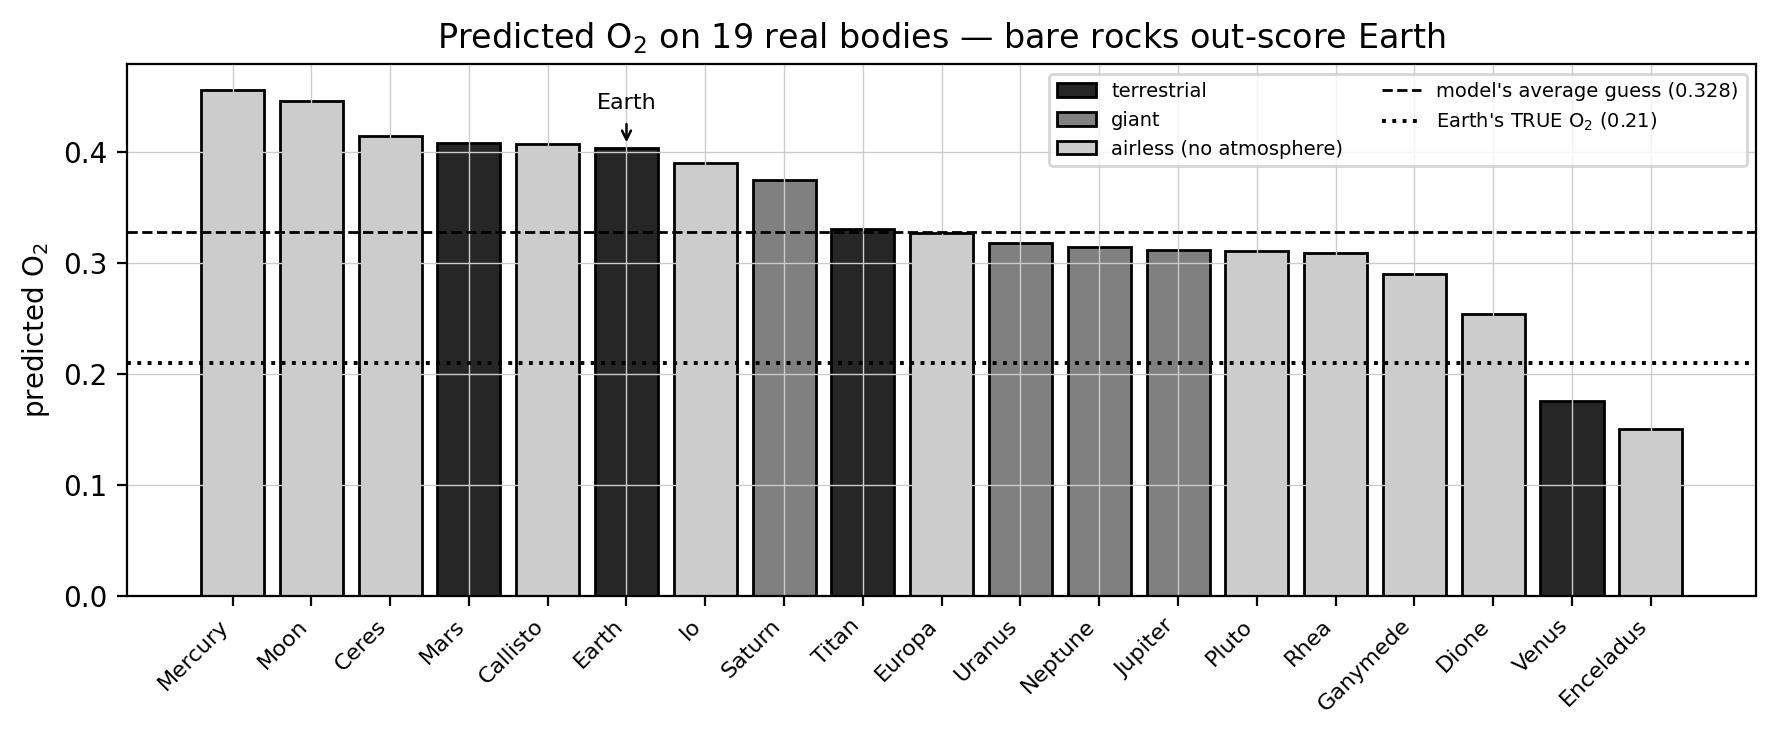
\includegraphics[width=\linewidth]{fig08_o2_fabrication.png}
\caption{Fabricated oxygen. Airless bodies are assigned oxygen abundances at or
above Earth's, driven by the training-set label prior.}
\label{fig:o2}
\end{figure}

\begin{figure}[t]
\centering
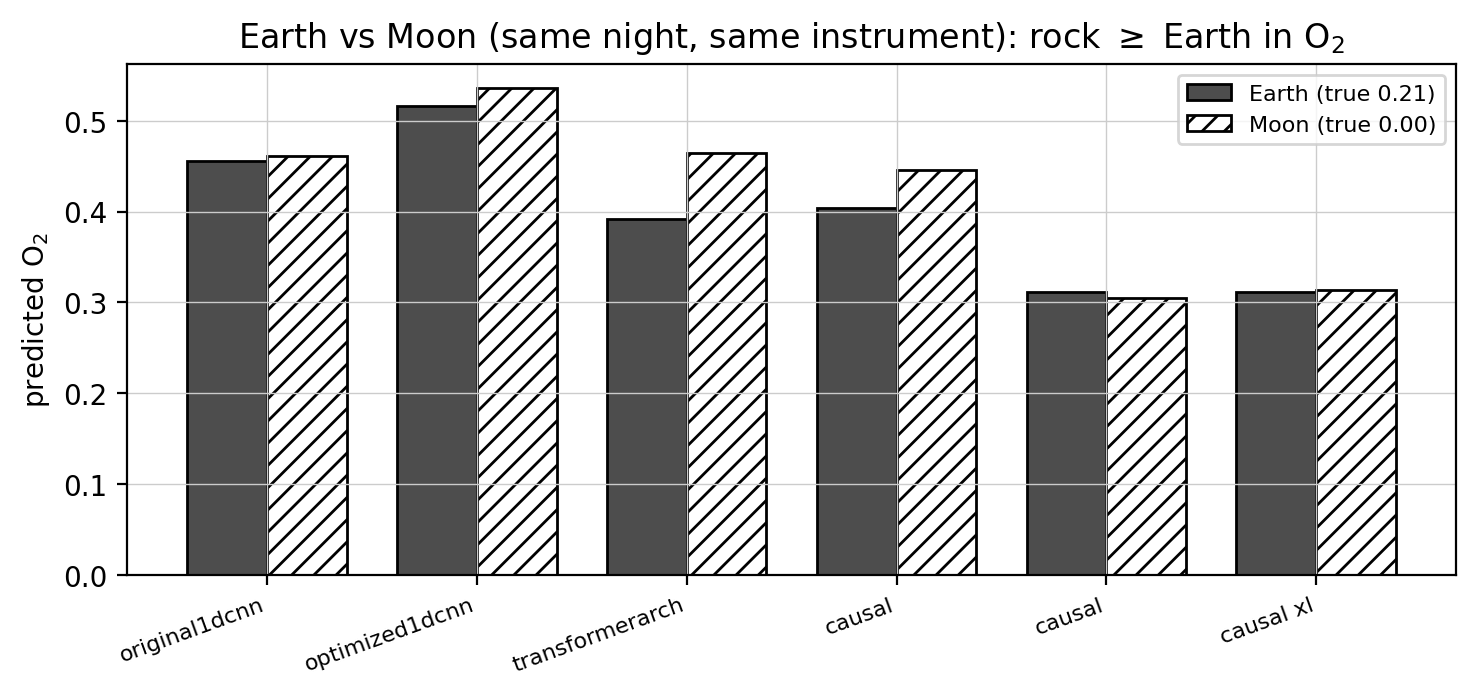
\includegraphics[width=\linewidth]{fig09_earth_vs_moon.png}
\caption{The matched Earth/Moon control. Most models fail to give Earth more
oxygen than its airless companion.}
\label{fig:earthmoon}
\end{figure}

\subsection{Inference-time correction}
\label{sec:corrections}

Continuum-twin nulling suppresses the fabrication without retraining
(Table~\ref{tab:null}, Figure~\ref{fig:null}). Subtracting the featureless-twin
prediction shrinks the mean fabricated abundances on airless bodies by a factor
of 20 to 80 (\ot: $0.341$ to $0.016$; \co: $0.351$ to $0.013$), raises the
Earth-versus-rock \ot{} AUROC from $0.64$ to $0.91$, and leaves methane detection
nearly intact ($1.00$ to $0.92$). The correction removes the prior-driven
baseline while preserving the feature-driven signal, and it needs no labels, so
it can be applied to any frozen model. It is a mitigation, not a cure: the
underlying model still encodes the biased prior, and the correction only cancels
its effect at the point of use.

\begin{table}[t]
\centering
\caption{Continuum-twin nulling on airless bodies (causal). Fabricated abundances
collapse, while methane survives.}
\label{tab:null}
\small
\begin{tabular}{@{}lcc@{}}
\toprule
Quantity & Raw & Nulled \\
\midrule
Mean $|$\ot$|$ on rocks & 0.341 & 0.016 \\
Mean $|$\co$|$ on rocks & 0.351 & 0.013 \\
\ot{} AUROC (Earth vs.\ rock) & 0.64 & 0.91 \\
\ch{} AUROC & 1.00 & 0.92 \\
\bottomrule
\end{tabular}
\end{table}

\begin{figure}[t]
\centering
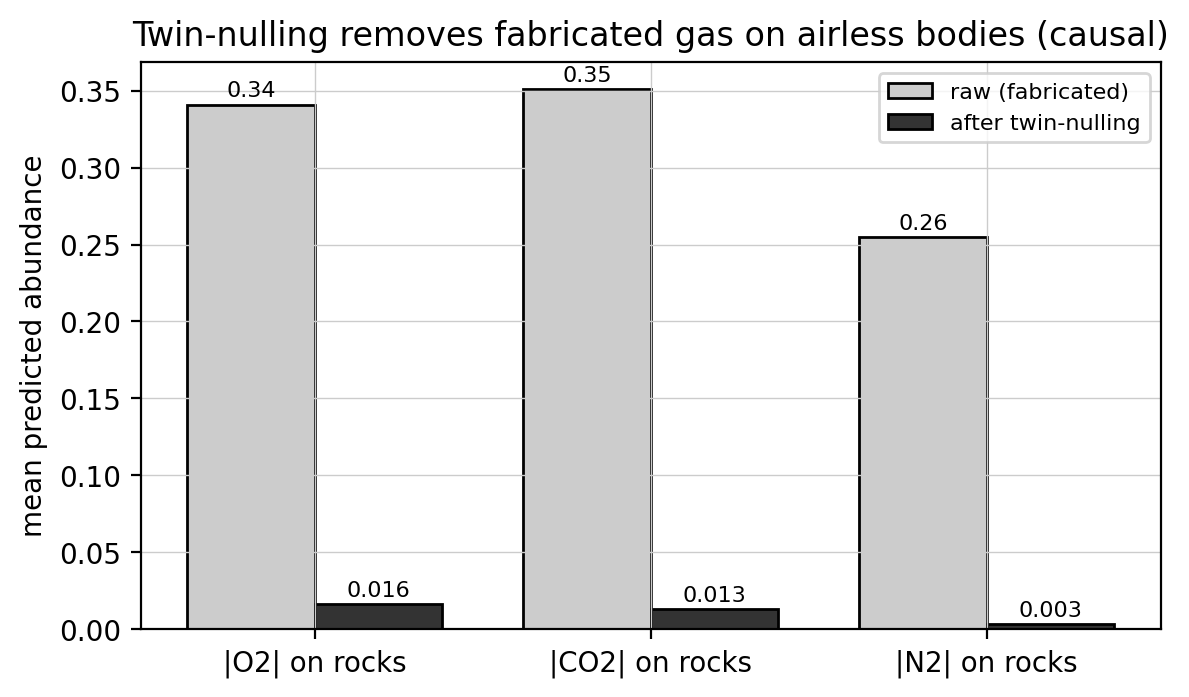
\includegraphics[width=\linewidth]{fig11_twin_nulling.png}
\caption{Continuum-twin nulling: prior-driven fabrication cancels per body while
genuine absorption survives.}
\label{fig:null}
\end{figure}

\subsection{Neural de-clouding: a negative result}
\label{sec:decloud_res}

The de-clouding module recovers 24 to 46\% of the accuracy lost to cloud
contamination, and it does so for held-out cloud morphologies it never saw in
training (Figure~\ref{fig:decloud}), which is encouraging in isolation. As a
usable component, however, it failed. It is not identity-safe: applied to
genuinely clear spectra it degrades accuracy, because it assumes clouds are
present and removes structure that is real, so it cannot be left always-on. Its
training clouds were parametric rather than physical, so the reconstructions did
not match the statistics of observed cloudy spectra, and, separately, folding
cloud contamination directly into retrieval training reduced accuracy rather than
improving robustness. We report the module as a negative result and keep cloud
removal separate from retrieval, applied only to spectra already known to be
cloudy.

\begin{figure}[t]
\centering
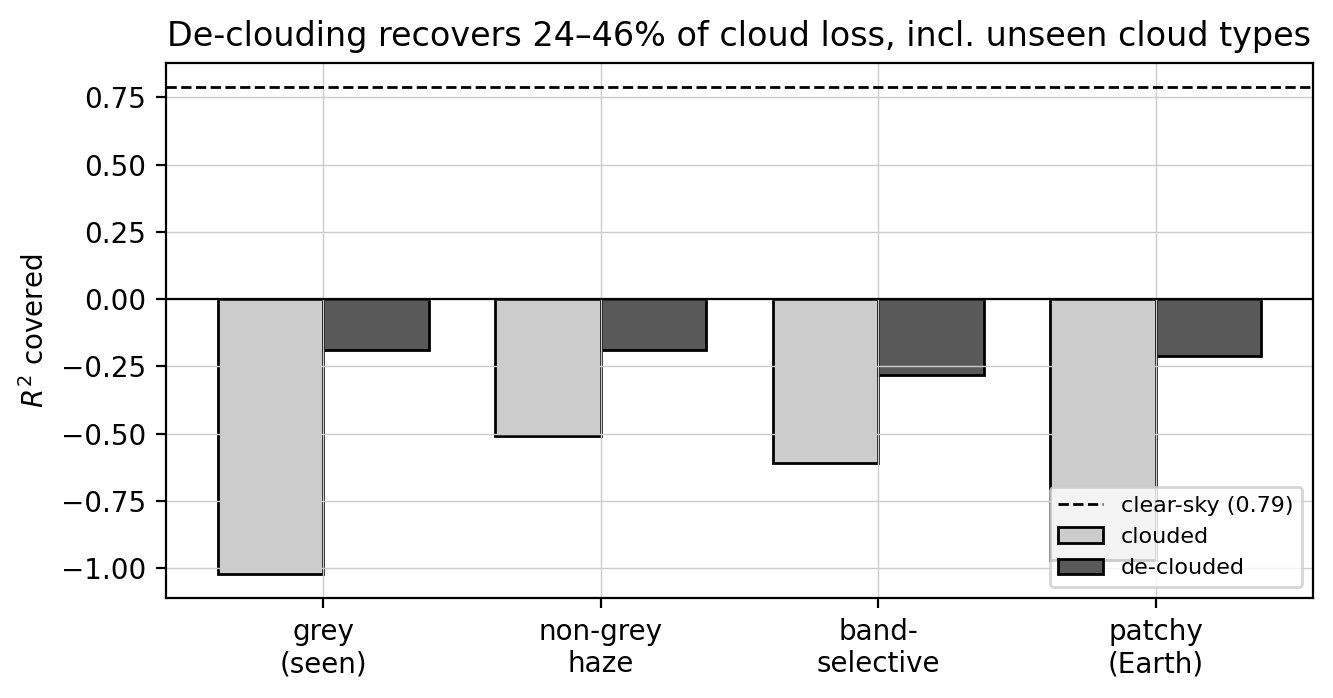
\includegraphics[width=\linewidth]{fig05_cloud_generalization.png}
\caption{De-clouding under seen (grey) and unseen cloud families. Accuracy is
partially recovered, but the module must not be applied to clear spectra.}
\label{fig:decloud}
\end{figure}

% ==================================================================
\section{Discussion}
% ==================================================================

The results are best read as a catalogue of the limitations of learned retrieval,
and of the controls that make those limitations visible.

\paragraph{Model size is not the lever.} Increasing capacity did not improve
accuracy: a 520k-parameter model matched a 36M-parameter one at the ceiling, and
enlarging the causal backbone hurt. What mattered was the input representation and
the training objective. Compact models are therefore preferable, being cheaper to
train, to audit, and to deploy, and effort is better spent on inputs, objectives,
and calibration than on scale. The causal augmentation gives the best ceiling and
robustness in our study, but the $+0.213$ gain is single-seed and measured at the
noiseless ceiling; at realistic exposures all architectures converge to a
photon-limited floor, so the augmentation buys accuracy only where signal-to-noise
is high.

\paragraph{Physics is a hard baseline on real data.} The one task the models
reliably perform on real spectra, methane detection, is matched by a
one-parameter band-depth ruler. For a single strong feature at high resolution,
transparent physics is competitive, and it should be the baseline any learned
method is measured against. The network's advantage is expected where the ruler
cannot easily go, in multi-gas joint retrieval, at lower resolution and lower
signal-to-noise, and in breaking degeneracies among correlated species. We have
characterised those regimes on synthetic data, but cannot yet demonstrate the
advantage on real spectra for want of suitable observations, and establishing it
is a defining goal for follow-up work.

\paragraph{Metrics must be read with physics.} The oxygen result is the clearest
warning. A model that fabricates the most important biosignature on airless rock
can still post a respectable aggregate $R^2$, because that metric rewards
reproducing the label distribution. Reliability requires pairing statistical
performance with physical controls, the airless-body false-positive test, the
occlusion check, and continuum nulling, and with honest uncertainty that, as we
show, holds only in-distribution. Much of the contribution of this paper is this
evaluation methodology rather than any single accuracy number, and the controls
are inexpensive: they reuse frozen models and require no new training.

\paragraph{The gap to real observations is wider than the cross-simulator gap.}
The cross-simulator collapse proved to be mostly removable covariate shift,
correctable by Adaptive Batch Normalisation without retraining, though a physics
residual remains. This is encouraging for transfer between simulators, but it does
not close the gap to real observations, whose domain shift also includes
instrumental systematics, viewing geometry, and cloud that no simulator contains.
The albedo-to-contrast conversion we use is itself an assumption; our detection
results are designed to be insensitive to it, but quantitative real-data retrieval
will require forward-modelling the observing conditions explicitly.

\paragraph{Recommendations.} For practitioners we draw three practical points.
Report accuracy at a realistic exposure, not only at a noiseless ceiling, and
state the assumed integration with every number. Include a false-positive control,
ideally airless bodies or otherwise featureless inputs, so that prior-driven
fabrication is caught before it is reported as a detection. And treat uncertainty
as valid only where it was calibrated, re-conditioning it under any shift in
resolution or noise. None of these require larger models or more training.

\paragraph{Limitations.} Several caveats bound our own conclusions. The
architecture and ablation numbers are single-seed, and at the shared budget some
tracks are undertrained, so the ceiling gaps should be confirmed with multiple
seeds at full budget. The real-data sample is small, 19 bodies with few of them
methane-bearing, so the detection AUROCs certify separation on this sample rather
than a population estimate. The cloud model is a parametric approximation, not
observed cloud physics. And we compare against Bayesian retrieval on cost and on
published accuracy, not yet by running nested sampling on the same real spectra.
None of these change the central, qualitative finding: synthetic accuracy
overstates real-world reliability, and physical controls are needed to detect the
difference.

% ==================================================================
\section{Conclusion}
% ==================================================================

We evaluated a family of six neural reflected-light retrieval models not only on
held-out synthetic spectra but on real telescope observations of 19 Solar-System
bodies, reporting accuracy at both a noiseless ceiling and a realistic single
exposure. The two differ by a factor of six, model size does not help,
cross-simulator transfer degrades, and the models fabricate oxygen on airless
bodies while detecting methane no better than a one-parameter physics ruler. A
compact counterfactually-augmented model achieves the best accuracy ceiling while
remaining far smaller than a conventional convolutional network, and a per-gas
ensemble of frozen models raises the ceiling further; continuum-twin nulling
suppresses the oxygen fabrication at inference time, without retraining and while
methane survives. The broader message is one of limitation rather than triumph:
machine-learning retrievals should be judged against physics and real
observations, with calibrated uncertainty, not against synthetic accuracy alone.
Running full Bayesian retrievals on the same real spectra, and confirming the
architecture and causal-augmentation effects across seeds and exposures, are the
priorities for future work.

% ==================================================================
\section*{Data and code availability}
% ==================================================================
\small
The synthetic library derives from INARA/PSG \citep{zorzan2025,villanueva2018},
and the real-data catalogue is the public Solar-System reflectance set of Madden
\& Kaltenegger \citep{madden2018}. All results were obtained from frozen model
checkpoints without retraining.

% ==================================================================
\begin{thebibliography}{99}
\small

\bibitem{gilbert2024} Gilbert-Janizek, B., et al. (2024). Reflected-light
characterisation of habitable-zone planets with future direct-imaging missions.

\bibitem{damiano2020} Damiano, M., \& Hu, R. (2020). Reflected-light spectroscopy
retrievals of terrestrial exoplanets. \textit{AJ}, 159, 175.

\bibitem{waldmann2016} Waldmann, I. P. (2016). Dreaming of atmospheres.
\textit{ApJ}, 820, 107.

\bibitem{marquez2018} M\'arquez-Neila, P., Fisher, C., Sznitman, R., \&
Heng, K. (2018). Supervised machine learning for analysing spectra of exoplanetary
atmospheres. \textit{Nature Astronomy}, 2, 719.

\bibitem{soboczenski2018} Soboczenski, F., et al. (2018). Bayesian deep learning
for exoplanet atmospheric retrieval. \textit{NeurIPS Workshop on Bayesian Deep
Learning}.

\bibitem{zingales2018} Zingales, T., \& Waldmann, I. P. (2018). ExoGAN:
retrieving exoplanetary atmospheres using deep convolutional generative
adversarial networks. \textit{AJ}, 156, 268.

\bibitem{cobb2019} Cobb, A. D., et al. (2019). An ensemble of Bayesian neural
networks for exoplanetary atmospheric retrieval. \textit{AJ}, 158, 33.

\bibitem{nixon2020} Nixon, M. C., \& Madhusudhan, N. (2020). Assessment of
supervised machine learning for atmospheric retrieval of exoplanets.
\textit{MNRAS}, 496, 269.

\bibitem{ardevol2022} Ard\'evol Mart\'inez, F., Min, M., Kamp, I., \&
Palmer, P. I. (2022). Convolutional neural networks as an alternative to Bayesian
retrievals for interpreting exoplanet transmission spectra. \textit{A\&A}, 662,
A9.

\bibitem{vasist2023} Vasist, M., et al. (2023). Neural posterior estimation for
exoplanetary atmospheric retrieval. \textit{A\&A}, 672, A147.

\bibitem{aubin2023} Aubin, M., et al. (2023). Simulation-based inference for
exoplanet atmospheric retrieval: winning the Ariel Data Challenge 2023 with
normalizing flows. \textit{NeurIPS ML4PS / ECML-PKDD}.

\bibitem{villanueva2018} Villanueva, G. L., et al. (2018). Planetary Spectrum
Generator. \textit{JQSRT}, 217, 86.

\bibitem{zorzan2025} Zorzan, et al. (2025). INARA: a machine-learning-ready data
set of synthetic reflected-light spectra for rocky exoplanets.

\bibitem{madden2018} Madden, J. H., \& Kaltenegger, L. (2018). A catalog of
Solar-System reflectance spectra for use as exoplanet analogues.
\textit{Astrobiology}, 18(12), 1559.

\end{thebibliography}

\end{document}
